% !TEX program = pdflatex
% ============================================================================
% Rapport de stage ingénieur — Plateforme de gestion des adhérents et des
% projets associatifs
% Compiles with pdflatex (2 passes needed for TOC/LOF/LOT/refs, as usual).
% ============================================================================
\documentclass[a4paper,12pt]{report}

% ------------------------------------------------------------------ Encoding
\usepackage[utf8]{inputenc}
\usepackage[T1]{fontenc}
\usepackage[french]{babel}
\usepackage{mathptmx} % Times-like text font, safe/standard on Overleaf

% ------------------------------------------------------------------ Layout
\usepackage[a4paper,margin=2.5cm]{geometry}
\usepackage{graphicx}
\usepackage{xcolor}
\usepackage{booktabs}
\usepackage{array}
\usepackage{longtable}
\usepackage{enumitem}
\usepackage{caption}
\usepackage{fancyhdr}
\usepackage{listings}
\usepackage{csquotes}
\usepackage{amsmath,amssymb}
\usepackage{float} % provides the [H] float specifier used by the figures below

% ------------------------------------------------------------------ TikZ
\usepackage{tikz}
\usetikzlibrary{arrows.meta,positioning,shapes.geometric,shapes.multipart,calc,fit,backgrounds}

% ------------------------------------------------------------------ Hyperref (load late)
\usepackage[hidelinks]{hyperref}

% ============================================================================
% Colors — approximate the reference report's blue corporate palette
% ============================================================================
\definecolor{reportblue}{RGB}{68,105,168}
\definecolor{reportbluedark}{RGB}{41,74,128}
\definecolor{lightblue}{RGB}{221,231,247}
\definecolor{lightblueborder}{RGB}{116,148,196}
\definecolor{panelgray}{RGB}{245,246,248}

\hypersetup{
  colorlinks=true,
  linkcolor=reportbluedark,
  citecolor=reportbluedark,
  urlcolor=reportbluedark,
  pdftitle={Plateforme de gestion des adhérents et des projets associatifs},
  pdfauthor={BOUDRAR Mohamed},
  pdfsubject={Rapport de stage ingénieur},
}

% ============================================================================
% Section numbering: I / II / III ... then 1 / 2 / 3 ... then a / b / c ...
% ============================================================================
\renewcommand{\thesection}{\Roman{section}}
\renewcommand{\thesubsection}{\arabic{subsection}}
\renewcommand{\thesubsubsection}{\alph{subsubsection}}

\usepackage{titlesec}
\titleformat{\section}
  {\color{reportblue}\Large\bfseries}{\thesection.}{0.6em}{}
\titlespacing*{\section}{0pt}{1.4em}{0.8em}

\titleformat{\subsection}
  {\color{reportblue}\large\bfseries}{\thesubsection.}{0.6em}{}
\titlespacing*{\subsection}{0pt}{1.1em}{0.6em}

\titleformat{\subsubsection}
  {\color{reportblue}\normalsize\bfseries}{\thesubsubsection.}{0.6em}{}
\titlespacing*{\subsubsection}{0pt}{0.9em}{0.4em}

% ============================================================================
% Page style: plain page numbers only, no running header — matches the
% reference report exactly (it has no repeating "Chapitre N" header, only a
% one-time recap line at the top of each chapter's first content page, added
% manually by \openchapter below).
% ============================================================================
\pagestyle{plain}
\renewcommand{\headrulewidth}{0pt}

% ============================================================================
% Custom "chapter" mechanism.
%
% \chapter itself is never used in this document. Using it would mean
% fighting titlesec/report.cls to suppress its default heading style while
% still keeping the figure/table "N.M" numbering and TOC entry it wires up
% automatically. Instead \openchapter below:
%   1. advances the real \chapter counter by hand (\stepcounter) — this is
%      what report.cls's own \thefigure/\thetable definitions key off, so
%      Figure/Table numbering ("3.1", "3.2", ...) keeps working exactly as
%      if \chapter had been called;
%   2. writes the TOC entry by hand (\addcontentsline);
%   3. draws a dedicated banner page ("CHAPITRE N :" + title), matching the
%      reference report's own chapter-opening pages;
%   4. prints the one-time "Chapitre N : Title" recap line + rule at the top
%      of the chapter's first real content page (never repeated afterwards
%      — the reference report does not use a repeating running header).
% ============================================================================
\makeatletter
\newcommand{\customtoc}{\@starttoc{toc}}
\newcommand{\customlof}{\@starttoc{lof}}
\newcommand{\customlot}{\@starttoc{lot}}
\makeatother

\newcommand{\openchapter}[1]{%
  \clearpage
  \stepcounter{chapter}
  \phantomsection
  \addcontentsline{toc}{chapter}{\thechapter.~~#1}
  \thispagestyle{empty}
  \vspace*{4.5cm}
  \begin{center}
    \colorbox{reportblue}{%
      \parbox{0.82\textwidth}{\centering\color{white}\Large\bfseries CHAPITRE \thechapter~:}%
    }\\[2.2cm]
    {\color{reportblue}\Huge\bfseries #1}
  \end{center}
  \clearpage
  \noindent{\large\bfseries Chapitre \thechapter\ : #1}\par
  \noindent\rule{\linewidth}{0.6pt}\par
  \vspace{0.8cm}
}

% Front-matter section (Remerciements, Table des matières, ...): same blue
% heading style, unnumbered, gets its own TOC entry, no chapter banner.
\newcommand{\frontsection}[1]{%
  \clearpage
  \phantomsection
  \addcontentsline{toc}{chapter}{#1}
  \thispagestyle{plain}
  {\color{reportblue}\Huge\bfseries #1}\par
  \vspace{1cm}
}

% ============================================================================
% Reusable TikZ styles for the diagrams (tree diagrams, class diagram,
% architecture pipeline, use-case diagram) — one consistent visual language
% across the whole report, mirroring the reference report's own style.
% ============================================================================
\tikzset{
  % --- Problem tree / solution tree (chapitre 2) -----------------------------
  treeeffect/.style={
    rectangle, rounded corners, draw=reportbluedark, fill=white,
    text width=4.8cm, align=center, minimum height=1cm, font=\scriptsize
  },
  treecore/.style={
    rectangle, rounded corners, draw=reportbluedark, fill=reportblue,
    text width=9.5cm, align=center, minimum height=1cm,
    font=\bfseries\small\color{white}
  },
  treecause/.style={
    rectangle, rounded corners, draw=lightblueborder, fill=lightblue,
    text width=3.7cm, align=center, minimum height=1.3cm, font=\scriptsize
  },
  treeroot/.style={
    rectangle, rounded corners, draw=lightblueborder, fill=panelgray,
    text width=3.7cm, align=center, minimum height=1.3cm, font=\scriptsize
  },
  % --- Use-case diagram (chapitre 3) ----------------------------------------
  % text width is kept at 2.9cm on purpose: the ellipse shape sizes itself so
  % that the text box fits *inside* the ellipse, which multiplies the width by
  % sqrt(2). 2.9cm of text therefore yields an ellipse ~4.2cm wide, which is
  % what the two-column layout of the diagram is built around.
  ucase/.style={
    ellipse, draw=reportblue, fill=lightblue, align=center,
    text width=2.9cm, inner sep=1pt, minimum height=1.15cm, font=\scriptsize
  },
  ucline/.style={draw=reportblue, semithick},
  actorline/.style={draw=reportbluedark, thick},
  sysboundary/.style={draw=reportbluedark, thick, rounded corners=2pt},
  % --- Class diagram (chapitre 3) -------------------------------------------
  umlclass/.style={
    rectangle split, rectangle split parts=2,
    rectangle split part fill={lightblue, white},
    draw=lightblueborder, thick, align=left, text width=3.3cm,
    inner sep=3pt, font=\scriptsize
  },
  rel/.style={draw=reportblue, thick},
  mult/.style={font=\tiny, inner sep=1.5pt, fill=white},
  % --- Architecture / états / divers ----------------------------------------
  archbox/.style={
    rectangle, rounded corners, draw=lightblueborder, fill=lightblue,
    text width=3.3cm, align=center, minimum height=1.6cm, font=\small
  },
  statebox/.style={
    rectangle, rounded corners, draw=reportblue, fill=lightblue,
    align=center, inner sep=6pt, font=\small
  },
  stateterm/.style={
    rectangle, rounded corners, draw=reportbluedark, fill=white,
    align=center, inner sep=6pt, font=\small, very thick
  },
  busline/.style={draw=reportblue, thick},
  bluearrow/.style={-{Latex[length=2.2mm]}, draw=reportblue, thick},
}

% A minimal UML-style stick-figure actor, used by the use-case diagram.
% #1 = position, e.g. (2,-3)   #2 = node name, for \draw references
% #3 = label, printed under the figure
% Besides drawing the figure, the macro declares an invisible node named #2
% covering the figure, so that (#2.east) / (#2.west) are usable anchors for
% the association lines.
\newcommand{\umlactor}[3]{%
  \begin{scope}[shift={#1}]
    \draw[actorline] (0,0.62) circle (0.2);
    \draw[actorline] (0,0.42) -- (0,-0.24);
    \draw[actorline] (-0.3,0.18) -- (0.3,0.18);
    \draw[actorline] (0,-0.24) -- (-0.26,-0.7);
    \draw[actorline] (0,-0.24) -- (0.26,-0.7);
    \node[align=center, text width=1.8cm, font=\scriptsize\bfseries,
          anchor=north, inner sep=1pt] at (0,-0.82) {#3};
  \end{scope}
  \node[draw=none, fill=none, inner sep=0pt, minimum width=0.62cm,
        minimum height=1.5cm] (#2) at #1 {};
}


% ============================================================================
% Listings style (for the API-contract code snippets in the annex)
% ============================================================================
\lstdefinelanguage{json}{
  showstringspaces=false,
  breaklines=true,
  sensitive=true,
  morekeywords={true,false,null},
  morestring=[b]",
  morecomment=[l]{//},
}

\lstdefinestyle{jsonstyle}{
  basicstyle=\ttfamily\small,
  backgroundcolor=\color{panelgray},
  frame=single,
  rulecolor=\color{lightblueborder},
  breaklines=true,
  columns=fullflexible,
  keywordstyle=\color{reportbluedark}\bfseries,
  commentstyle=\color{gray},
  stringstyle=\color{reportbluedark},
  showstringspaces=false,
}
\lstset{style=jsonstyle}

\captionsetup{labelfont={bf,color=reportbluedark},font=small,margin=1cm}

% ============================================================================
\begin{document}

% ============================================================================
% Cover page — mirrors the reference report's layout: blue frame border,
% two logo placeholders (top-left: school; top-right: host organism), an
% institutional banner, a blue "STAGE INGÉNIEUR D'ÉTUDES" box, project
% title + subtitle, and a Réalisé par / Superviseur / Tuteur académique
% block. Everything institution-specific is left as an explicit
% placeholder, matching Chapitre 1 (which is not written yet) and the
% reference's own "À préciser" convention.
% ============================================================================
\begin{titlepage}
\thispagestyle{empty}

\noindent\begin{minipage}[t]{0.48\textwidth}
  \raggedright
  \fbox{\parbox[c][1.6cm][c]{4.2cm}{%
    \centering
    
\includegraphics[width=3.8cm,height=1.3cm,keepaspectratio]{images.png}
}}
\end{minipage}%
\hfill
\begin{minipage}[t]{0.48\textwidth}
  \raggedleft
  \fbox{\parbox[c][1.6cm][c]{4.2cm}{%
    \centering
    
\includegraphics[width=3.8cm,height=1.3cm,keepaspectratio]{logo.png}
}}
\end{minipage}

\vspace{2cm}

\begin{center}
  {\bfseries\large CYCLE INGÉNIEUR --- Ecole Polytechnique D'Agadir}\\[0.3cm]
  {\bfseries\large FILIÈRE Génie Informatique}

  \vspace{1.8cm}

  \colorbox{reportblue}{%
    \parbox[c][1.3cm][c]{9.5cm}{\centering\color{white}\Large\bfseries STAGE INGÉNIEUR D'ÉTUDES}%
  }

  \vspace{2.4cm}
  {\Huge\bfseries Plateforme de gestion des abonnés \\[0.2cm] et des projets d'une association}

  \vspace{0.6cm}

  {\itshape\large
    Conception et développement d'une application web pour la gestion\\
    des cotisations, des comités de projets et des opérations financières\\
    d'une association
  }

  \vspace{3cm}
\end{center}

\noindent
\begin{minipage}[t]{0.48\textwidth}
  {\color{reportbluedark}\bfseries Réalisé par :}\\
  BOUDRAR Mohamed
\end{minipage}%
\hfill
\begin{minipage}[t]{0.48\textwidth}

    {\color{reportbluedark}\bfseries Encadré par :}\\
    À préciser

  \end{minipage}

\vfill
\vspace{2.5cm}

\begin{center}
  {\bfseries Année universitaire 2026 - 2027}
\end{center}

\vspace{1cm}

\end{titlepage}


\pagenumbering{arabic}
\setcounter{page}{1}

\frontsection{Remerciements}

Je tiens à exprimer ma profonde gratitude à \textbf{Omni Networks} pour m’avoir offert l’opportunité de réaliser ce stage au sein de son environnement professionnel, ainsi que pour la confiance qui m’a été accordée tout au long de cette expérience. Cette immersion m’a permis de mettre en pratique mes connaissances, d’acquérir de nouvelles compétences et de mieux appréhender les exigences du monde professionnel.

\vspace{0.5cm}

J’adresse mes sincères remerciements à mon superviseur de stage pour son encadrement, sa disponibilité, ses conseils pertinents et son accompagnement tout au long de la réalisation de ce projet. Ses orientations et son expertise ont largement contribué à la réussite de ce travail et à la richesse de mon expérience.

\vspace{0.5cm}

Je tiens également à remercier mes amis pour leur soutien, leurs encouragements et leur présence tout au long de cette période. Leur bienveillance et leur motivation ont été précieuses et m’ont accompagné durant les différentes étapes de ce projet.

\vspace{0.5cm}

Enfin, j’adresse mes sincères remerciements à l’ensemble des collaborateurs de \textbf{Omni Networks}, ainsi qu’à toutes les personnes qui, de près ou de loin, ont contribué au bon déroulement de mon stage et à la réalisation de ce projet.

\vspace{0.5cm}

\textbf{À toutes et à tous, j’adresse ma sincère reconnaissance.}

\frontsection{Table des matières}
\customtoc

\frontsection{Table des illustrations}
{\large\bfseries\color{reportbluedark} Figures}\par\vspace{0.3cm}
\customlof
\vspace{1cm}
{\large\bfseries\color{reportbluedark} Tableaux}\par\vspace{0.3cm}
\customlot

\frontsection{Introduction Générale}

Dans le cadre de ma formation en cycle ingénieur, ce stage de fin d'année porte sur la conception et le développement d'une application web dédiée à la gestion des abonnés et des projets d'une association. L'objectif est de proposer une solution centralisée permettant de faciliter le suivi des adhérents, des abonnements, des projets associatifs et des différentes opérations financières qui leur sont associées.

\vspace{0.5cm}

Le fonctionnement de l'association repose notamment sur les cotisations annuelles de ses abonnés ainsi que sur différentes sources de financement destinées à la réalisation de projets à caractère social, tels que le forage de puits ou la construction et la rénovation de bâtiments. Pour chaque projet, un comité est constitué afin d'assurer son suivi de sa création jusqu'à sa clôture. Les membres de ce comité doivent pouvoir enregistrer les dons, les dépenses et les différentes pièces justificatives liées aux opérations réalisées.

\vspace{0.5cm}

La gestion de ces informations nécessite une organisation rigoureuse et une bonne traçabilité des opérations financières. L'application développée doit ainsi permettre de centraliser ces données, de gérer les droits d'accès des différents membres, de conserver les justificatifs associés aux opérations et de faciliter la préparation des rapports des projets. Elle doit également permettre à chaque abonné de consulter son propre historique, notamment ses abonnements, ses dons et les éventuelles sommes restant dues.

\vspace{0.5cm}

La problématique de ce stage consiste donc à concevoir une solution adaptée aux besoins de l'association, permettant d'améliorer la gestion, le suivi et la traçabilité de ses activités tout en simplifiant l'accès aux informations pour les différents acteurs.

\vspace{0.5cm}

Ce rapport présente les différentes étapes de réalisation de ce projet. Le premier chapitre présente l'organisme d'accueil et le contexte du stage. Le deuxième chapitre est consacré à l'étude et à l'analyse des besoins. Enfin, le troisième chapitre présente la conception et la mise en œuvre de la solution développée.


% ============================================================================
% CHAPITRE 1 — Présentation de l'organisme & du sujet
% Structure alignée sur la table des matières cible
% ============================================================================
\openchapter{Présentation de l'organisme \& du sujet}

\section{Introduction}

Ce premier chapitre présente le cadre général dans lequel s'est déroulé ce stage de fin d'année. Il commence par une présentation de l'organisme d'accueil afin de situer l'environnement professionnel dans lequel le projet a été réalisé. Il expose ensuite le contexte et l'organisation du projet, avant de détailler le sujet de stage, sa problématique, la méthode de gestion adoptée, l'équipe impliquée et le planning de réalisation.

\section{Présentation de l'organisme d'accueil}

\textbf{Omni Networks} est une entreprise fondée à Agadir par une équipe d'ingénieurs spécialisée dans le développement de logiciels. Forte de plus de 20 ans d'expérience dans le domaine du développement de solutions métiers, l'entreprise met son expertise au service des entreprises afin de répondre à leurs différents besoins en matière de gestion et de fonctionnement.

L'activité de Omni Networks repose principalement sur la conception et le développement de solutions logicielles adaptées aux besoins de ses clients. L'entreprise accompagne ainsi ses clients dans l'évolution et l'amélioration de leurs outils et processus, quels que soient leur taille ou leur domaine d'activité.

Animée par une démarche orientée vers l'innovation et l'amélioration continue, Omni Networks s'appuie sur trois principes essentiels : \textbf{créer, innover et améliorer}. Cette approche lui permet de développer et de faire évoluer des produits de gestion destinés à accompagner durablement les entreprises dans leurs activités.

\section{Contexte et organisation du projet}

Le projet réalisé au cours de ce stage s'inscrit dans le développement d'une solution de gestion destinée à une association dont les activités reposent principalement sur les cotisations de ses abonnés et sur différentes sources de financement. L'association réalise notamment des projets à caractère social, tels que le forage de puits, ainsi que la construction et la rénovation de mosquées, de maisons pour veuves et d'orphelins. Les projets peuvent être financés par les cotisations des abonnés, les contributions des membres et des bienfaiteurs, ainsi que par des dons de l'État ou d'autres associations.

L'organisation de l'association repose sur plusieurs catégories de membres, parmi lesquelles le président, le vice-président, le trésorier, le vice-trésorier, le secrétaire général, le vice-secrétaire général et les conseillers. Les membres du bureau sont également considérés comme des abonnés de l'association.

Pour chaque projet, le bureau constitue un comité composé de membres de l'association. Ce comité est chargé d'assurer le suivi du projet de son lancement jusqu'à sa clôture. Selon leurs responsabilités et leurs droits, les membres du comité peuvent enregistrer les différentes opérations liées au projet, notamment les dons des adhérents, les paiements, les dépenses ainsi que les documents justificatifs tels que les reçus et les factures.

Dans ce contexte, le projet consiste à mettre en place une application permettant de centraliser ces informations et d'organiser leur gestion selon les rôles des différents utilisateurs. La solution doit également permettre de conserver les justificatifs associés aux opérations, de faciliter la préparation des rapports de clôture des projets et de permettre aux abonnés de consulter leur propre historique, comprenant leurs abonnements, leurs dons et les éventuelles sommes restant dues.

\section{Présentation du sujet de stage}

\subsection{Titre du projet}

\textbf{Conception et développement d'une plateforme web de gestion des abonnés et des projets d'une association}

\subsection{Problématique}

La gestion des abonnés, des cotisations et des projets d'une association implique le suivi d'un grand nombre d'informations : paiements des abonnements, dons, dépenses, factures, reçus et autres pièces justificatives. À cela s'ajoute la nécessité de suivre les projets individuellement et de permettre aux différents membres d'intervenir selon leurs responsabilités.

Le principal enjeu du projet est donc de centraliser ces informations au sein d'une même plateforme, tout en garantissant une gestion adaptée aux rôles des utilisateurs et une traçabilité des opérations réalisées. La solution doit également faciliter le suivi financier des projets, la conservation des documents justificatifs et la préparation des rapports de clôture.

Une autre problématique concerne les abonnés eux-mêmes. Chaque abonné doit pouvoir accéder à son historique afin de consulter ses abonnements, ses dons ainsi que les éventuelles sommes restant dues à l'association.

La problématique générale peut ainsi être formulée de la manière suivante :

\begin{quote}
\textit{Comment concevoir et développer une plateforme web permettant de centraliser la gestion des abonnés et des projets d'une association, d'assurer la traçabilité des opérations financières et de faciliter l'accès aux informations selon les rôles des différents utilisateurs ?}
\end{quote}

\subsection{Méthode de gestion de projet}

Compte tenu de la nature du projet et du fait que sa réalisation a été effectuée individuellement et à distance, une approche itérative et progressive a été adoptée. Le développement a été organisé en plusieurs étapes, allant de l'analyse des besoins et de la définition des fonctionnalités à la conception, au développement, aux tests et aux corrections.

Cette organisation a permis d'avancer progressivement sur les différentes fonctionnalités de l'application, tout en intégrant les ajustements nécessaires au fur et à mesure de l'avancement du projet. Les échanges réguliers avec le superviseur de stage ont permis de valider les orientations prises et de recueillir les remarques nécessaires à l'amélioration de la solution.

\subsection{Équipe de projet}

La réalisation de ce projet a été effectuée individuellement et à distance. En tant que stagiaire développeur, j'ai assuré l'ensemble des activités liées à la réalisation de la solution, notamment l'analyse des besoins, la conception, la modélisation, le développement, les tests ainsi que la correction des anomalies.

Le projet a néanmoins bénéficié d'un encadrement à deux niveaux. Le superviseur de stage a assuré le suivi professionnel du projet, en apportant ses orientations et ses recommandations tout au long de sa réalisation. Le tuteur académique a, quant à lui, assuré le suivi pédagogique du stage et veillé au bon déroulement du travail dans le cadre de la formation d'ingénieur.

L'organisation à distance a reposé principalement sur des échanges réguliers avec l'encadrement, permettant de suivre l'avancement du projet, de discuter des choix réalisés et de valider progressivement les différentes étapes.

\subsection{Planning du projet}

Le projet a été réalisé progressivement selon plusieurs phases, depuis l'analyse initiale des besoins jusqu'à la finalisation de l'application. Les principales étapes sont les suivantes :

\begin{enumerate}
    \item \textbf{Analyse des besoins} : étude du fonctionnement de l'association, identification des acteurs et définition des besoins fonctionnels et techniques.
    \item \textbf{Conception} : modélisation du système, définition de l'architecture de la solution et conception de la base de données.
    \item \textbf{Développement} : implémentation progressive des différentes fonctionnalités de l'application et intégration des composants du système.
    \item \textbf{Tests fonctionnels et techniques} : réalisation de tests sur les fonctionnalités développées afin de vérifier leur bon fonctionnement dans différents scénarios d'utilisation et d'identifier les éventuelles anomalies.
    \item \textbf{Correction et amélioration} : correction des anomalies détectées lors des tests et amélioration progressive des fonctionnalités et de l'interface.
    \item \textbf{Finalisation} : stabilisation de l'application, amélioration de l'expérience utilisateur et préparation de la documentation du projet.
\end{enumerate}

Ces phases n'ont pas été strictement séquentielles : conformément à la démarche itérative décrite plus haut, le développement, les tests et les corrections se sont recouverts d'une itération à l'autre, chaque nouveau module fonctionnel étant testé et corrigé avant que le suivant ne soit abordé. Le récapitulatif suivant associe à chaque phase son objectif principal et le livrable correspondant.

\begin{center}
\small
\begin{tabular}{@{}p{3.6cm}p{4.6cm}p{5.2cm}@{}}
\toprule
\textbf{Phase} & \textbf{Objectif principal} & \textbf{Livrable} \\
\midrule
Analyse des besoins & Comprendre le fonctionnement de l'association & Liste des acteurs et des besoins fonctionnels \\
\addlinespace[2pt]
Conception & Structurer la solution avant le codage & Modèle de données, architecture technique \\
\addlinespace[2pt]
Développement & Implémenter les modules fonctionnels & API REST et interfaces web opérationnelles \\
\addlinespace[2pt]
Tests fonctionnels et techniques & Vérifier le comportement attendu & Anomalies identifiées et documentées \\
\addlinespace[2pt]
Correction et amélioration & Traiter les anomalies et affiner l'ergonomie & Version corrigée et stabilisée \\
\addlinespace[2pt]
Finalisation & Consolider et documenter la solution & Application finalisée et documentation \\
\bottomrule
\end{tabular}
\end{center}

\section{Conclusion}

Ce chapitre a permis de présenter le cadre général du stage, l'organisme d'accueil ainsi que le contexte dans lequel s'inscrit le projet. Le fonctionnement de l'association, son organisation et les principaux besoins liés à la gestion des abonnés et des projets ont également été présentés.

Le sujet du stage, sa problématique ainsi que l'organisation du travail ont ensuite été définis. Le projet étant réalisé individuellement et à distance, une démarche progressive a été adoptée, allant de l'analyse des besoins jusqu'au développement, aux tests et à la finalisation de la solution.

Le chapitre suivant sera consacré à l'étude préalable du projet. Il permettra d'approfondir l'analyse des besoins, d'identifier les différents acteurs et de définir les fonctionnalités attendues de la solution.
% ============================================================================
% CHAPITRE 2 — Étude préalable
% Structure alignée sur la table des matières cible
% ============================================================================
\openchapter{Étude préalable}

\section{Introduction}

Avant de détailler la conception et la réalisation du projet (chapitre~3), ce
chapitre propose une étude préalable du sujet : pourquoi une plateforme dédiée
est nécessaire, à qui elle s'adresse, quelles approches alternatives existent
et pourquoi elles ne répondent pas au besoin, ainsi que le cadrage logique du
problème à résoudre.

\section{Pourquoi ce projet, à qui il s'adresse, approches existantes}

\subsection{Pourquoi ce projet ?}

Le fonctionnement d'une association repose sur deux flux qui doivent rester
étroitement liés : la cotisation annuelle que chaque adhérent verse selon les
résultats de l'assemblée générale, et les projets associatifs (forage de
puits, construction ou rénovation de mosquées, aide aux veuves et aux
orphelins, etc.) que l'association finance grâce à ces cotisations, aux dons
de ses propres membres ou de bienfaiteurs, ainsi qu'aux dons de l'État et
d'autres associations. Avant de lancer un projet, le bureau constitue un
comité chargé de le mener de A à Z, et chaque membre du comité doit pouvoir
saisir les opérations qui relèvent de son rôle : montant des dons reçus,
reçus de paiement, factures des fournisseurs. À la fin du projet, le comité
doit produire un rapport détaillant les entrées et les dépenses, accompagné
des factures, bons et copies de chèques ; le bureau, de son côté, doit
présenter un rapport annuel aux adhérents.

Tant que ce suivi repose sur des tableurs et des dossiers papier, il devient
rapidement fragile : rien n'empêche une saisie en double ou une perte de
justificatif, rien ne garantit qu'un membre du comité ne voie que ce qui
relève de son rôle, et un adhérent n'a aucun moyen simple de connaître sa
propre situation (cotisation payée, dons effectués, solde dû). Un système
qui centralise ces opérations, applique des droits différenciés selon le rôle
de chaque membre et conserve une traçabilité systématique des justificatifs
répond directement à cette limite.

\subsection{À qui s'adresse ce projet ?}

Le projet s'adresse à l'ensemble des parties prenantes d'une association
telle que décrite dans son cahier des charges : le \textbf{bureau de
l'association} (président, vice-président, trésorier, vice-trésorier,
secrétaire général, vice-secrétaire général et conseillers), qui pilote
l'association et supervise l'ensemble des projets et des cotisations ; les
\textbf{comités de projet}, constitués ponctuellement par le bureau pour
mener un projet donné, dont les membres saisissent les opérations financières
de ce projet selon leur rôle au sein du comité ; et les \textbf{adhérents}
(abonnés), qui financent l'association par leur cotisation et peuvent, selon
le cas, être aussi des donateurs ou des membres de comité. Les huit rôles
identifiés et leurs droits respectifs sont détaillés au chapitre~3
(section~III).

\subsection{Approches existantes}

Trois grandes familles d'outils permettent, en théorie, de gérer les
cotisations et les projets d'une association :

\begin{itemize}
  \item \textbf{Le suivi manuel (tableurs et papier)} — rapide à mettre en
    place, sans coût de développement, mais sans droits d'accès
    différenciés, sans traçabilité systématique des justificatifs, et sans
    consultation en libre-service pour l'adhérent : chaque demande de
    situation personnelle repasse par le bureau.

  \item \textbf{Un logiciel de comptabilité générique} — apporte une
    tenue de compte robuste, mais n'est pas structuré autour de la notion
    de \emph{comité de projet} : il ne distingue pas nativement les droits
    d'un trésorier de comité de ceux d'un simple membre, ne rattache pas un
    don ou une dépense à un projet et à son cycle de vie propre (comité
    constitué, financement réuni, projet actif, clôturé), et ne propose
    aucun espace personnel pour un adhérent. Son coût de licence est en
    outre disproportionné pour une association à but non lucratif.

  \item \textbf{Une plateforme de gestion associative sur mesure} —
    conçue autour des besoins réels exprimés dans le cahier des charges du
    stage : cotisations annuelles, projets avec comités dédiés, saisie des
    opérations selon le rôle de chaque membre, justificatifs numérisés
    (reçus, factures, photos de chèques ou d'ordres de virement), rapport de
    clôture par projet et historique personnel pour chaque adhérent.
\end{itemize}

C'est cette troisième approche qui a été retenue : elle seule permet de
modéliser fidèlement la structure à deux niveaux de l'association (rôle
global dans le bureau, rôle local dans un comité de projet) et de répondre
point par point aux exigences du cahier des charges, ce qu'aucun outil
générique ne permet sans détournement de son usage prévu.

\section{Cadrage logique}

\subsection{Problématique et enjeux}

L'enjeu du projet est double : offrir au bureau et aux comités de projet un
outil qui centralise et sécurise la gestion des cotisations et des
opérations financières, tout en restant suffisamment simple pour être adopté
par des utilisateurs non spécialistes de l'informatique.

\subsection{Arbre à problèmes et arbre à solutions}

\begin{figure}[H]
  \centering
  \begin{tikzpicture}[node distance=0.9cm and 0.5cm]
    \node[problembox] (p1) {Suivi des cotisations et des dons dispersé sur papier et tableurs};
    \node[problembox, right=of p1] (p2) {Aucune séparation des droits selon le rôle dans le comité de projet};
    \node[problembox, right=of p2] (p3) {Absence de traçabilité centralisée des justificatifs (reçus, factures, chèques)};
    \node[concbox, below=1.4cm of p2] (pc) {Gestion associative peu fiable et chronophage};
    \draw[bluearrow] (p1.south) -- (pc.north -| p1.south);
    \draw[bluearrow] (p2.south) -- (pc.north);
    \draw[bluearrow] (p3.south) -- (pc.north -| p3.south);
  \end{tikzpicture}
  \caption{Arbre à problèmes : causes principales d'une gestion associative peu fiable.}
  \label{fig:arbre-problemes}
\end{figure}

\begin{figure}[H]
  \centering
  \begin{tikzpicture}[node distance=0.9cm and 0.5cm]
    \node[problembox] (s1) {Plateforme centralisée de gestion des cotisations et des dons};
    \node[problembox, right=of s1] (s2) {Droits d'accès différenciés par rôle global et par rôle de comité};
    \node[problembox, right=of s2] (s3) {Traçabilité systématique des opérations avec justificatifs numérisés};
    \node[concbox, below=1.4cm of s2] (sc) {Système de gestion associative fiable et traçable};
    \draw[bluearrow] (s1.south) -- (sc.north -| s1.south);
    \draw[bluearrow] (s2.south) -- (sc.north);
    \draw[bluearrow] (s3.south) -- (sc.north -| s3.south);
  \end{tikzpicture}
  \caption{Arbre à solutions : réponses apportées aux causes identifiées.}
  \label{fig:arbre-solutions}
\end{figure}

\subsection{Objectif général du projet}

Concevoir et développer une plateforme web permettant au bureau de
l'association de gérer ses adhérents, ses cotisations annuelles et ses
projets associatifs ; aux comités constitués pour chaque projet de saisir les
opérations financières selon les droits de leurs membres ; et à chaque
adhérent de consulter en libre-service son propre historique (cotisation,
dons, solde dû) — le tout avec une traçabilité complète des opérations et de
leurs justificatifs.

\section{Conclusion}

Ce chapitre a posé le cadre logique du projet : pourquoi une plateforme
dédiée est nécessaire, à qui elle s'adresse, pourquoi les approches
existantes n'y répondent pas, et quel objectif général elle poursuit. Le
chapitre suivant détaille les missions et travaux réalisés : la modélisation
conceptuelle du système retenu et sa mise en \oe uvre informatique.
% ============================================================================
% CHAPITRE 3 — Missions et travaux réalisés
% ============================================================================
\openchapter{Missions et travaux réalisés}

\section{Introduction}

Ce chapitre présente la spécification fonctionnelle du système, les acteurs
identifiés et leurs rôles, la structure des données manipulées, l'architecture
technique retenue, l'environnement de développement, le détail des
fonctionnalités implémentées, ainsi que les interfaces développées pour
chaque profil d'utilisateur.

\section{Spécification fonctionnelle}

À partir du cahier des charges du stage, le système doit permettre :

\begin{itemize}
  \item la \textbf{gestion des adhérents} : création d'un profil adhérent,
    consultation et mise à jour de ses coordonnées, suppression ;
  \item la \textbf{gestion des cotisations annuelles} : enregistrement d'un
    paiement de cotisation avec son reçu, vérification par un rôle financier
    du bureau, suivi d'une cotisation \emph{due} par adhérent et par année
    (montant dû, montant payé, solde, statut), avec génération automatique
    des cotisations et détection des retards ;
  \item la \textbf{gestion des projets associatifs} : création d'un projet,
    constitution d'un comité dédié, suivi de son cycle de vie jusqu'à sa
    clôture ou son annulation ;
  \item les \textbf{comités par projet} : chaque comité regroupe des membres
    avec un rôle propre au projet (président de comité, trésorier,
    secrétaire, membre), indépendant du rôle global de la personne dans
    l'association, et saisit les opérations financières du projet selon ce
    rôle ;
  \item le \textbf{workflow des dons et des dépenses} avec approbation :
    toute entrée ou sortie d'argent sur un projet passe par un circuit
    brouillon~$\rightarrow$~soumis~$\rightarrow$~approuvé ou rejeté, avec
    justificatif obligatoire (reçu, facture, photo de chèque ou d'ordre de
    virement) ;
  \item les \textbf{rapports de clôture} : à la fin d'un projet, un rapport
    PDF récapitulant les entrées, les dépenses et les justificatifs est
    généré automatiquement, et un rapport association-wide (adhérents,
    cotisations, projets, cotisations dues) est disponible en PDF et Excel
    à tout moment pour le bureau ;
  \item la \textbf{consultation en libre-service}, pour chaque adhérent, de
    son propre historique : cotisations, dons effectués, solde dû.
\end{itemize}

\section{Identification des acteurs et rôles}

Le cahier des charges distingue le \emph{rôle global} d'une personne dans
l'association (président, vice-président, trésorier, vice-trésorier,
secrétaire général, vice-secrétaire général, conseiller, ou simple adhérent)
de son éventuel \emph{rôle dans un comité de projet} (président de comité,
trésorier de comité, secrétaire, membre) : les membres du bureau de
l'association sont eux-mêmes des adhérents, et un adhérent sans rôle global
particulier peut être trésorier d'un comité de projet donné.


\begin{figure}[H]
    \centering
    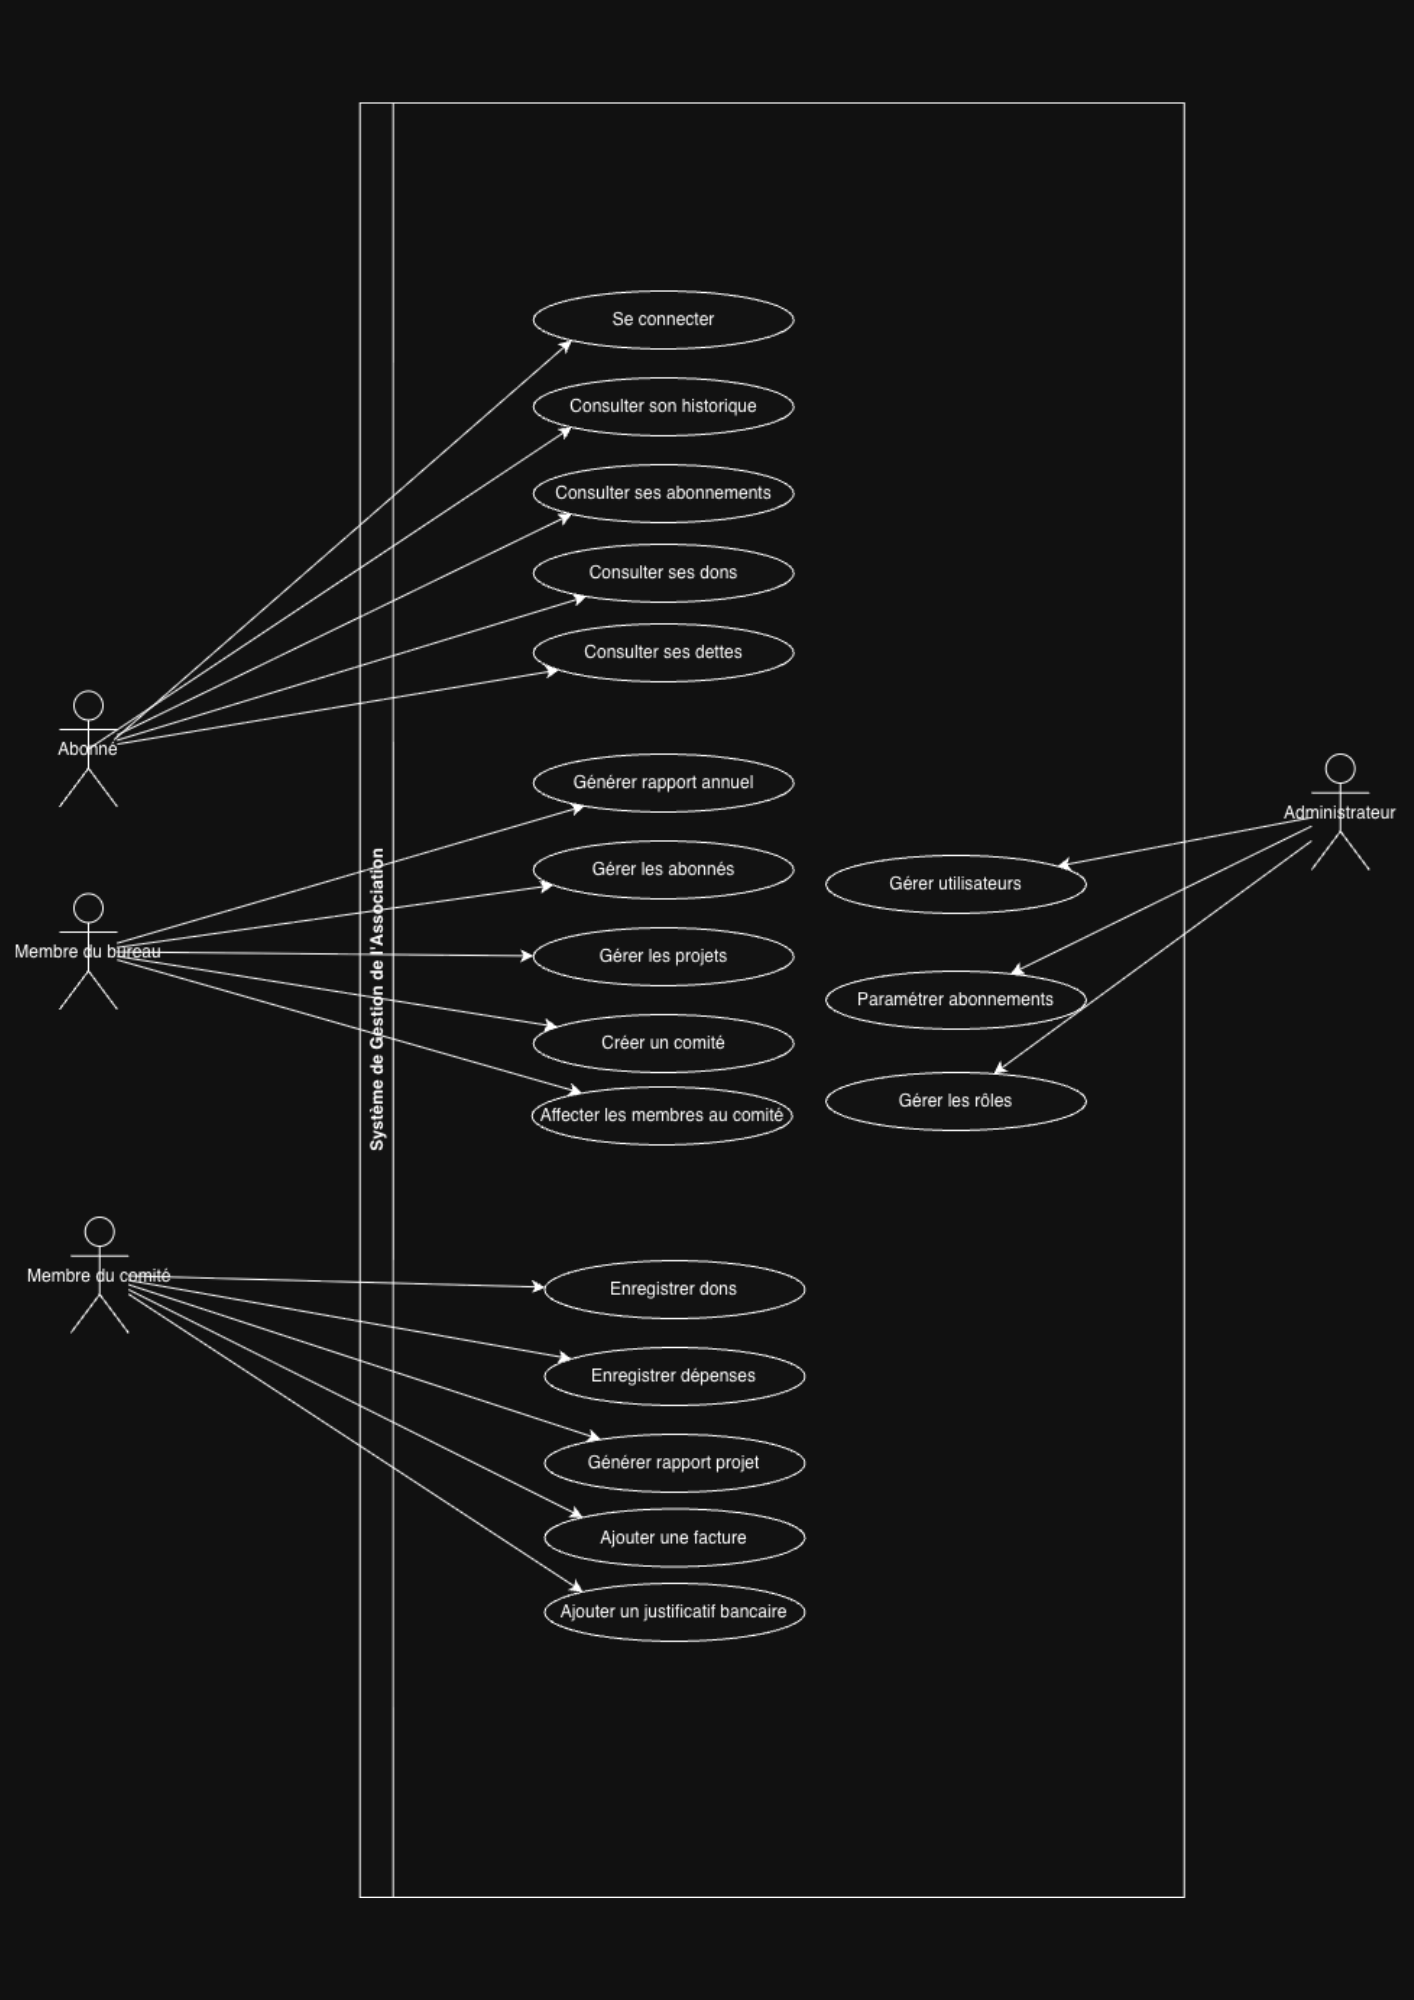
\includegraphics[width=\textwidth]{use-case.png}
    \caption{Diagramme de cas d'utilisation}
    \label{fig:use-case}
\end{figure}


Le détail complet des droits par rôle global (adhérents, cotisations, dues,
projets, dons, dépenses) figure dans la matrice de l'Annexe~B.

\section{Structure des données}

La figure~\ref{fig:classes} présente une vue simplifiée des principales
entités manipulées par le système et de leurs relations. \texttt{Member}
représente un adhérent (lié à un compte \texttt{User} pour l'authentification,
non représenté ici) ; \texttt{Due} porte le montant dû par un adhérent pour
une année donnée, réglé par une ou plusieurs \texttt{Subscription} (paiements
de cotisation) ; \texttt{Project} centralise le cycle de vie d'un projet, ses
\texttt{Donation}, ses \texttt{Expense} et les transferts de fonds
(\texttt{ProjectFundAllocation}) qui lui sont alloués ; \texttt{CommitteeAssignment}
est l'historique, jamais supprimé, des rôles tenus par un adhérent au sein du
comité d'un projet ; \texttt{ProjectReport} porte le rapport de clôture
généré à la fin d'un projet ; \texttt{Notification} peut être rattachée à
n'importe laquelle des autres entités (relation polymorphique).

\begin{figure}[htbp]
  \centering
  \begin{tikzpicture}[node distance=0.9cm and 0.9cm, every node/.style={font=\scriptsize}]
    \node[entitybox] (member) {\textbf{Member}\\ user\_id, phone, address};
    \node[entitybox, right=2.6cm of member] (project) {\textbf{Project}\\ name, budget, status, phase};

    \node[entitybox, below=of member] (subscription) {\textbf{Subscription}\\ member\_id, due\_id, amount, status};
    \node[entitybox, left=1.1cm of subscription] (due) {\textbf{Due}\\ member\_id, year, amount\_due,\\ balance, status};

    \node[entitybox, below=of project] (committee) {\textbf{CommitteeAssignment}\\ project\_id, member\_id,\\ committee\_role, action};
    \node[entitybox, right=1.1cm of committee] (allocation) {\textbf{ProjectFundAllocation}\\ project\_id, amount, allocation\_date};

    \node[entitybox, below=1.6cm of subscription] (donation) {\textbf{Donation}\\ member\_id, project\_id,\\ amount, status};
    \node[entitybox, right=1.1cm of donation] (expense) {\textbf{Expense}\\ project\_id, amount,\\ status};
    \node[entitybox, right=1.1cm of expense] (report) {\textbf{ProjectReport}\\ project\_id, file\_path, summary};

    \node[entitybox, below=2.4cm of project] (notification) {\textbf{Notification}\\ user\_id, type,\\ subject\_type, subject\_id};

    \draw[bluearrow] (member.east) -- (subscription.north);
    \draw[bluearrow] (member.west) .. controls +(-0.8,0) and +(-0.8,0) .. (due.north);
    \draw[bluearrow] (subscription.west) -- node[above,font=\tiny]{règle} (due.east);
    \draw[bluearrow] (member.south) .. controls +(0,-2) and +(2,2.4) .. (donation.north);
    \draw[bluearrow] (member.east) .. controls +(3.2,-1) and +(3.4,4) .. (committee.north east);

    \draw[bluearrow] (project.south) -- (committee.north);
    \draw[bluearrow] (project.east) .. controls +(1,-1) and +(0,1.4) .. (allocation.north);
    \draw[bluearrow] (project.south) .. controls +(0,-2.2) and +(2,3.4) .. (donation.north east);
    \draw[bluearrow] (project.south) .. controls +(1,-2.6) and +(0,2.4) .. (expense.north);
    \draw[bluearrow] (project.south) .. controls +(2,-2.8) and +(0,2.6) .. (report.north);
    \draw[bluearrow] (project.south) .. controls +(-1.4,-4.6) and +(1,3.4) .. (notification.east);
    \draw[bluearrow] (donation.south) .. controls +(0,-1) and +(-1,1) .. (notification.north west);
  \end{tikzpicture}
  \caption{Diagramme de classes simplifié du système.}
  \label{fig:classes}
\end{figure}

\section{Architecture technique}

Le système est bâti selon une architecture web classique en trois niveaux :
une interface web (React) qui consomme une API REST (Laravel), elle-même
adossée à une base de données relationnelle (MySQL) et à un espace de
stockage de fichiers pour les justificatifs. La figure~\ref{fig:architecture}
résume cette organisation.

\begin{figure}[htbp]
  \centering
  \begin{tikzpicture}[node distance=0.7cm]
    \node[archbox, text width=9.5cm, minimum height=1.6cm] (front)
      {\textbf{Interface web} --- React~19 + Vite, Tailwind~CSS,\\ Recharts, TomTom Maps SDK, ExcelJS};
    \node[archbox, below=of front, text width=9.5cm, minimum height=2.1cm] (api)
      {\textbf{API REST} --- Laravel~13\\ Authentification par jeton (Sanctum) $\cdot$ Rôles et permissions (Spatie)\\ Policies par ressource $\cdot$ Génération PDF (dompdf) $\cdot$ Export Excel};
    \node[archbox, below=of api, text width=4.5cm, minimum height=1.4cm] (db)
      {\textbf{Base de données}\\ MySQL};
    \node[archbox, right=1cm of db, text width=4.5cm, minimum height=1.4cm] (storage)
      {\textbf{Stockage fichiers}\\ Reçus, factures, rapports PDF};

    \draw[bluearrow] (front.south) -- node[right,font=\scriptsize]{HTTP / JSON} (api.north);
    \draw[bluearrow] (api.south) -- (db.north -| api.south);
    \draw[bluearrow] (api.south) -- (storage.north -| api.south);
  \end{tikzpicture}
  \caption{Architecture générale de la plateforme.}
  \label{fig:architecture}
\end{figure}

\section{Environnement de développement}

Le tableau~\ref{tab:outils} présente les principaux outils et technologies
utilisés pour la réalisation du projet.

\begin{center}
\begin{longtable}{@{}p{2.6cm}p{11.5cm}@{}}
\toprule
\textbf{Outil} & \textbf{Rôle dans le projet} \\
\midrule
\endhead
\colorbox{lightblue}{\parbox[c][0.9cm][c]{2.3cm}{\centering\bfseries React}} &
  Bibliothèque JavaScript utilisée pour l'interface web : tableau de bord,
  pages de gestion des adhérents, des projets, des finances et des rapports,
  toutes consommant l'API REST du backend. \\[0.4cm]
\colorbox{lightblue}{\parbox[c][0.9cm][c]{2.3cm}{\centering\bfseries Laravel}} &
  Framework PHP utilisé pour l'API REST : routage, validation des requêtes,
  authentification, autorisation et accès aux données. \\[0.4cm]
\colorbox{lightblue}{\parbox[c][0.9cm][c]{2.3cm}{\centering\bfseries MySQL}} &
  Système de gestion de base de données relationnelle stockant les
  adhérents, cotisations, projets, dons, dépenses et journaux d'activité. \\[0.4cm]
\colorbox{lightblue}{\parbox[c][0.9cm][c]{2.3cm}{\centering\bfseries Tailwind CSS}} &
  Framework CSS utilitaire pour la mise en forme de l'interface web. \\[0.4cm]
\colorbox{lightblue}{\parbox[c][0.9cm][c]{2.3cm}{\centering\bfseries Sanctum}} &
  Extension Laravel gérant l'authentification par jeton (bureau et portail
  adhérent), utilisée pour sécuriser chaque appel à l'API. \\[0.4cm]
\colorbox{lightblue}{\parbox[c][0.9cm][c]{2.3cm}{\centering\bfseries Spatie Permission}} &
  Bibliothèque de gestion des rôles et permissions, à la base du contrôle
  d'accès par rôle global décrit à la section~III. \\[0.4cm]
\colorbox{lightblue}{\parbox[c][0.9cm][c]{2.3cm}{\centering\bfseries dompdf}} &
  Génération des rapports PDF (rapport de clôture de projet, rapports
  association, reçus). \\[0.4cm]
\colorbox{lightblue}{\parbox[c][0.9cm][c]{2.3cm}{\centering\bfseries Maatwebsite Excel}} &
  Export des rapports association (adhérents, cotisations, projets, dues)
  au format Excel. \\[0.4cm]
\colorbox{lightblue}{\parbox[c][0.9cm][c]{2.3cm}{\centering\bfseries TomTom Maps SDK}} &
  Sélection et affichage de la localisation géographique d'un projet sur une
  carte interactive. \\
\bottomrule
\caption{Principaux outils et technologies utilisés pour le développement.}
\label{tab:outils}
\end{longtable}
\end{center}

\section{Fonctionnalités implémentées}

\subsection{Cycle de vie des projets}

Un projet suit un cycle de vie à cinq états administratifs, illustré à la
figure~\ref{fig:lifecycle}. Le passage de \emph{brouillon} à \emph{comité
constitué} se produit automatiquement dès qu'un premier membre est affecté au
comité du projet ; le passage à \emph{financement réuni} se produit
automatiquement dès la première allocation de fonds. Le démarrage
(\emph{actif}) et la clôture (\emph{terminé}) sont des actions explicites du
président ou du président de comité. Un projet peut être annulé depuis
n'importe quel état non terminal. Une fois \emph{terminé} ou \emph{annulé},
un projet devient définitivement en lecture seule et son comité est dissous.

\begin{figure}[htbp]
  \centering
  \begin{tikzpicture}[node distance=1.6cm, every node/.style={font=\small}]
    \node[statebox] (draft) {Brouillon};
    \node[statebox, right=of draft] (committee) {Comité constitué};
    \node[statebox, right=of committee] (funding) {Financement réuni};
    \node[statebox, right=of funding] (active) {Actif};
    \node[statebox, right=of active] (done) {Terminé};
    \node[statebox, below=1.2cm of active] (cancelled) {Annulé};

    \draw[bluearrow] (draft) -- node[above,font=\scriptsize]{1\textsuperscript{er} membre affecté} (committee);
    \draw[bluearrow] (committee) -- node[above,font=\scriptsize]{1\textsuperscript{re} allocation} (funding);
    \draw[bluearrow] (funding) -- node[above,font=\scriptsize]{démarrage} (active);
    \draw[bluearrow] (active) -- node[above,font=\scriptsize]{clôture} (done);
    \draw[bluearrow] (draft.south) -- (cancelled.west);
    \draw[bluearrow] (committee.south) -- (cancelled.north west);
    \draw[bluearrow] (funding.south) -- (cancelled.north);
    \draw[bluearrow] (active.south) -- (cancelled.north);
  \end{tikzpicture}
  \caption{Cycle de vie administratif d'un projet.}
  \label{fig:lifecycle}
\end{figure}

Un second axe, indépendant, suit l'avancement \emph{réel} du projet
(\emph{planification} $\rightarrow$ \emph{préparation} $\rightarrow$ \emph{en
cours} $\rightarrow$ \emph{finition} $\rightarrow$ \emph{terminé}) : le
président de comité soumet une demande de passage à l'étape suivante, avec
justificatifs, que le président ou le vice-président approuve ou rejette.
Cet avancement ne peut jamais être modifié directement, ni sauter une étape.

\subsection{Workflow d'approbation des dons et des dépenses}

Chaque don et chaque dépense saisi par un comité suit le même circuit
d'approbation (figure~\ref{fig:approbation}) : un membre habilité du comité
(président ou trésorier de comité) crée l'enregistrement à l'état
\emph{brouillon}, le complète avec son justificatif (reçu ou facture) puis le
soumet. Seul un rôle financier du bureau (président, trésorier ou
vice-trésorier) peut ensuite l'approuver ou le rejeter ; la personne qui a
saisi l'opération ne peut jamais approuver sa propre saisie. Un rejet précise
son motif et son type (justificatif à remplacer, ou détails erronés) : dans
le premier cas, le comité peut corriger le justificatif et resoumettre le
même enregistrement ; dans le second, l'enregistrement reste figé et une
nouvelle saisie doit être créée. Pour une dépense uniquement, une fois
approuvée, elle peut être marquée \emph{payée} — un état terminal.

\begin{figure}[htbp]
  \centering
  \begin{tikzpicture}[node distance=1.7cm, every node/.style={font=\small}]
    \node[statebox] (draft) {Brouillon};
    \node[statebox, right=of draft] (pending) {Soumis};
    \node[statebox, above right=0.9cm and 1.7cm of pending] (approved) {Approuvé};
    \node[statebox, below right=0.9cm and 1.7cm of pending] (rejected) {Rejeté};
    \node[statebox, right=1.7cm of approved] (paid) {Payé\\ \scriptsize(dépenses)};

    \draw[bluearrow] (draft) -- (pending);
    \draw[bluearrow] (pending) -- (approved);
    \draw[bluearrow] (pending) -- (rejected);
    \draw[bluearrow] (approved) -- (paid);
    \draw[bluearrow] (rejected.north) to[out=110,in=-110] node[left,font=\scriptsize]{justificatif corrigé} (pending.south);
  \end{tikzpicture}
  \caption{Workflow d'approbation des dons et des dépenses.}
  \label{fig:approbation}
\end{figure}

\subsection{Système de comités et historique}

Avant tout projet, le bureau constitue un comité et affecte à chacun de ses
membres un rôle propre au projet (président de comité, trésorier, secrétaire
ou membre) — ce rôle détermine les droits de saisie décrits ci-dessus, quel
que soit le rôle global de la personne dans l'association. Chaque affectation,
remplacement, démission, retrait ou dissolution (à la clôture ou à
l'annulation du projet) est conservé dans un historique qui n'est jamais
purgé, consultable projet par projet, avec la date, l'auteur de l'action et
son motif.

\subsection{Cotisations annuelles et suivi des dues}

En complément du paiement d'une cotisation (\texttt{Subscription}), chaque
adhérent dispose d'un solde dû par année (\texttt{Due}) : montant dû, montant
réglé, solde restant, statut (en attente, partiel, payé, en retard, exonéré).
Ce solde est recalculé automatiquement à chaque paiement vérifié qui lui est
rattaché ; le rattachement lui-même est automatique dès la création d'un
paiement de cotisation. Une tâche planifiée génère les dues de l'année en
cours pour chaque adhérent et bascule au statut \emph{en retard} celles dont
l'échéance est dépassée sans solde nul. Un rôle financier du bureau peut, à
titre exceptionnel, exonérer une cotisation due.

\subsection{Rapports de clôture et rapports association}

À la clôture d'un projet, un rapport PDF est généré automatiquement :
total des dons, des dépenses, des fonds alloués, solde reversé à
l'association, accompagné du détail de chaque opération. Indépendamment,
le bureau dispose à tout moment de rapports association-wide (adhérents,
cotisations, projets, cotisations dues), téléchargeables en PDF ou au format
Excel.

\subsection{Journal d'activité}

Chaque création, modification ou action de workflow (soumission, approbation,
rejet, paiement) est journalisée automatiquement. Le journal est consultable
sous forme de recherche/filtre par utilisateur, projet, type d'entité, action
et période ; sa portée dépend du rôle du lecteur : le président, le
vice-président et le trésorier voient l'ensemble de l'activité, les autres
rôles du bureau ne voient que celle des projets auxquels ils sont affectés,
et un simple adhérent n'y a pas accès.

\subsection{Centre de notifications}

Chaque événement significatif (cotisation à vérifier, don ou dépense en
attente d'approbation, projet clôturé, cotisation en retard, affectation à un
comité, etc.) génère une notification pour les personnes concernées : la
personne à l'origine de l'action, les rôles habilités à la traiter, ou les
deux. Chaque notification renvoie directement vers l'écran concerné.

\subsection{Authentification}

Deux mécanismes d'authentification coexistent, contre le même jeton d'accès :
les membres du bureau se connectent par email et mot de passe ; un adhérent
se connecte par un code numérique à six chiffres (« passkey »), délivré
automatiquement par email la première fois que sa cotisation est vérifiée par
le bureau. Les deux profils accèdent ensuite au même tableau de bord, dont le
contenu s'adapte à leur rôle et à leurs éventuelles affectations de comité.

\section{Interfaces développées}

Cette section présente les principales interfaces développées, une par
profil d'utilisateur ou par domaine fonctionnel.

\subsection{Tableau de bord du président}

Le tableau de bord du président centralise les indicateurs clés de
l'association : fonds disponibles, cotisations, projets par état, comités,
ainsi que les listes d'approbations en attente.

\begin{figure}[htbp]
  \centering
  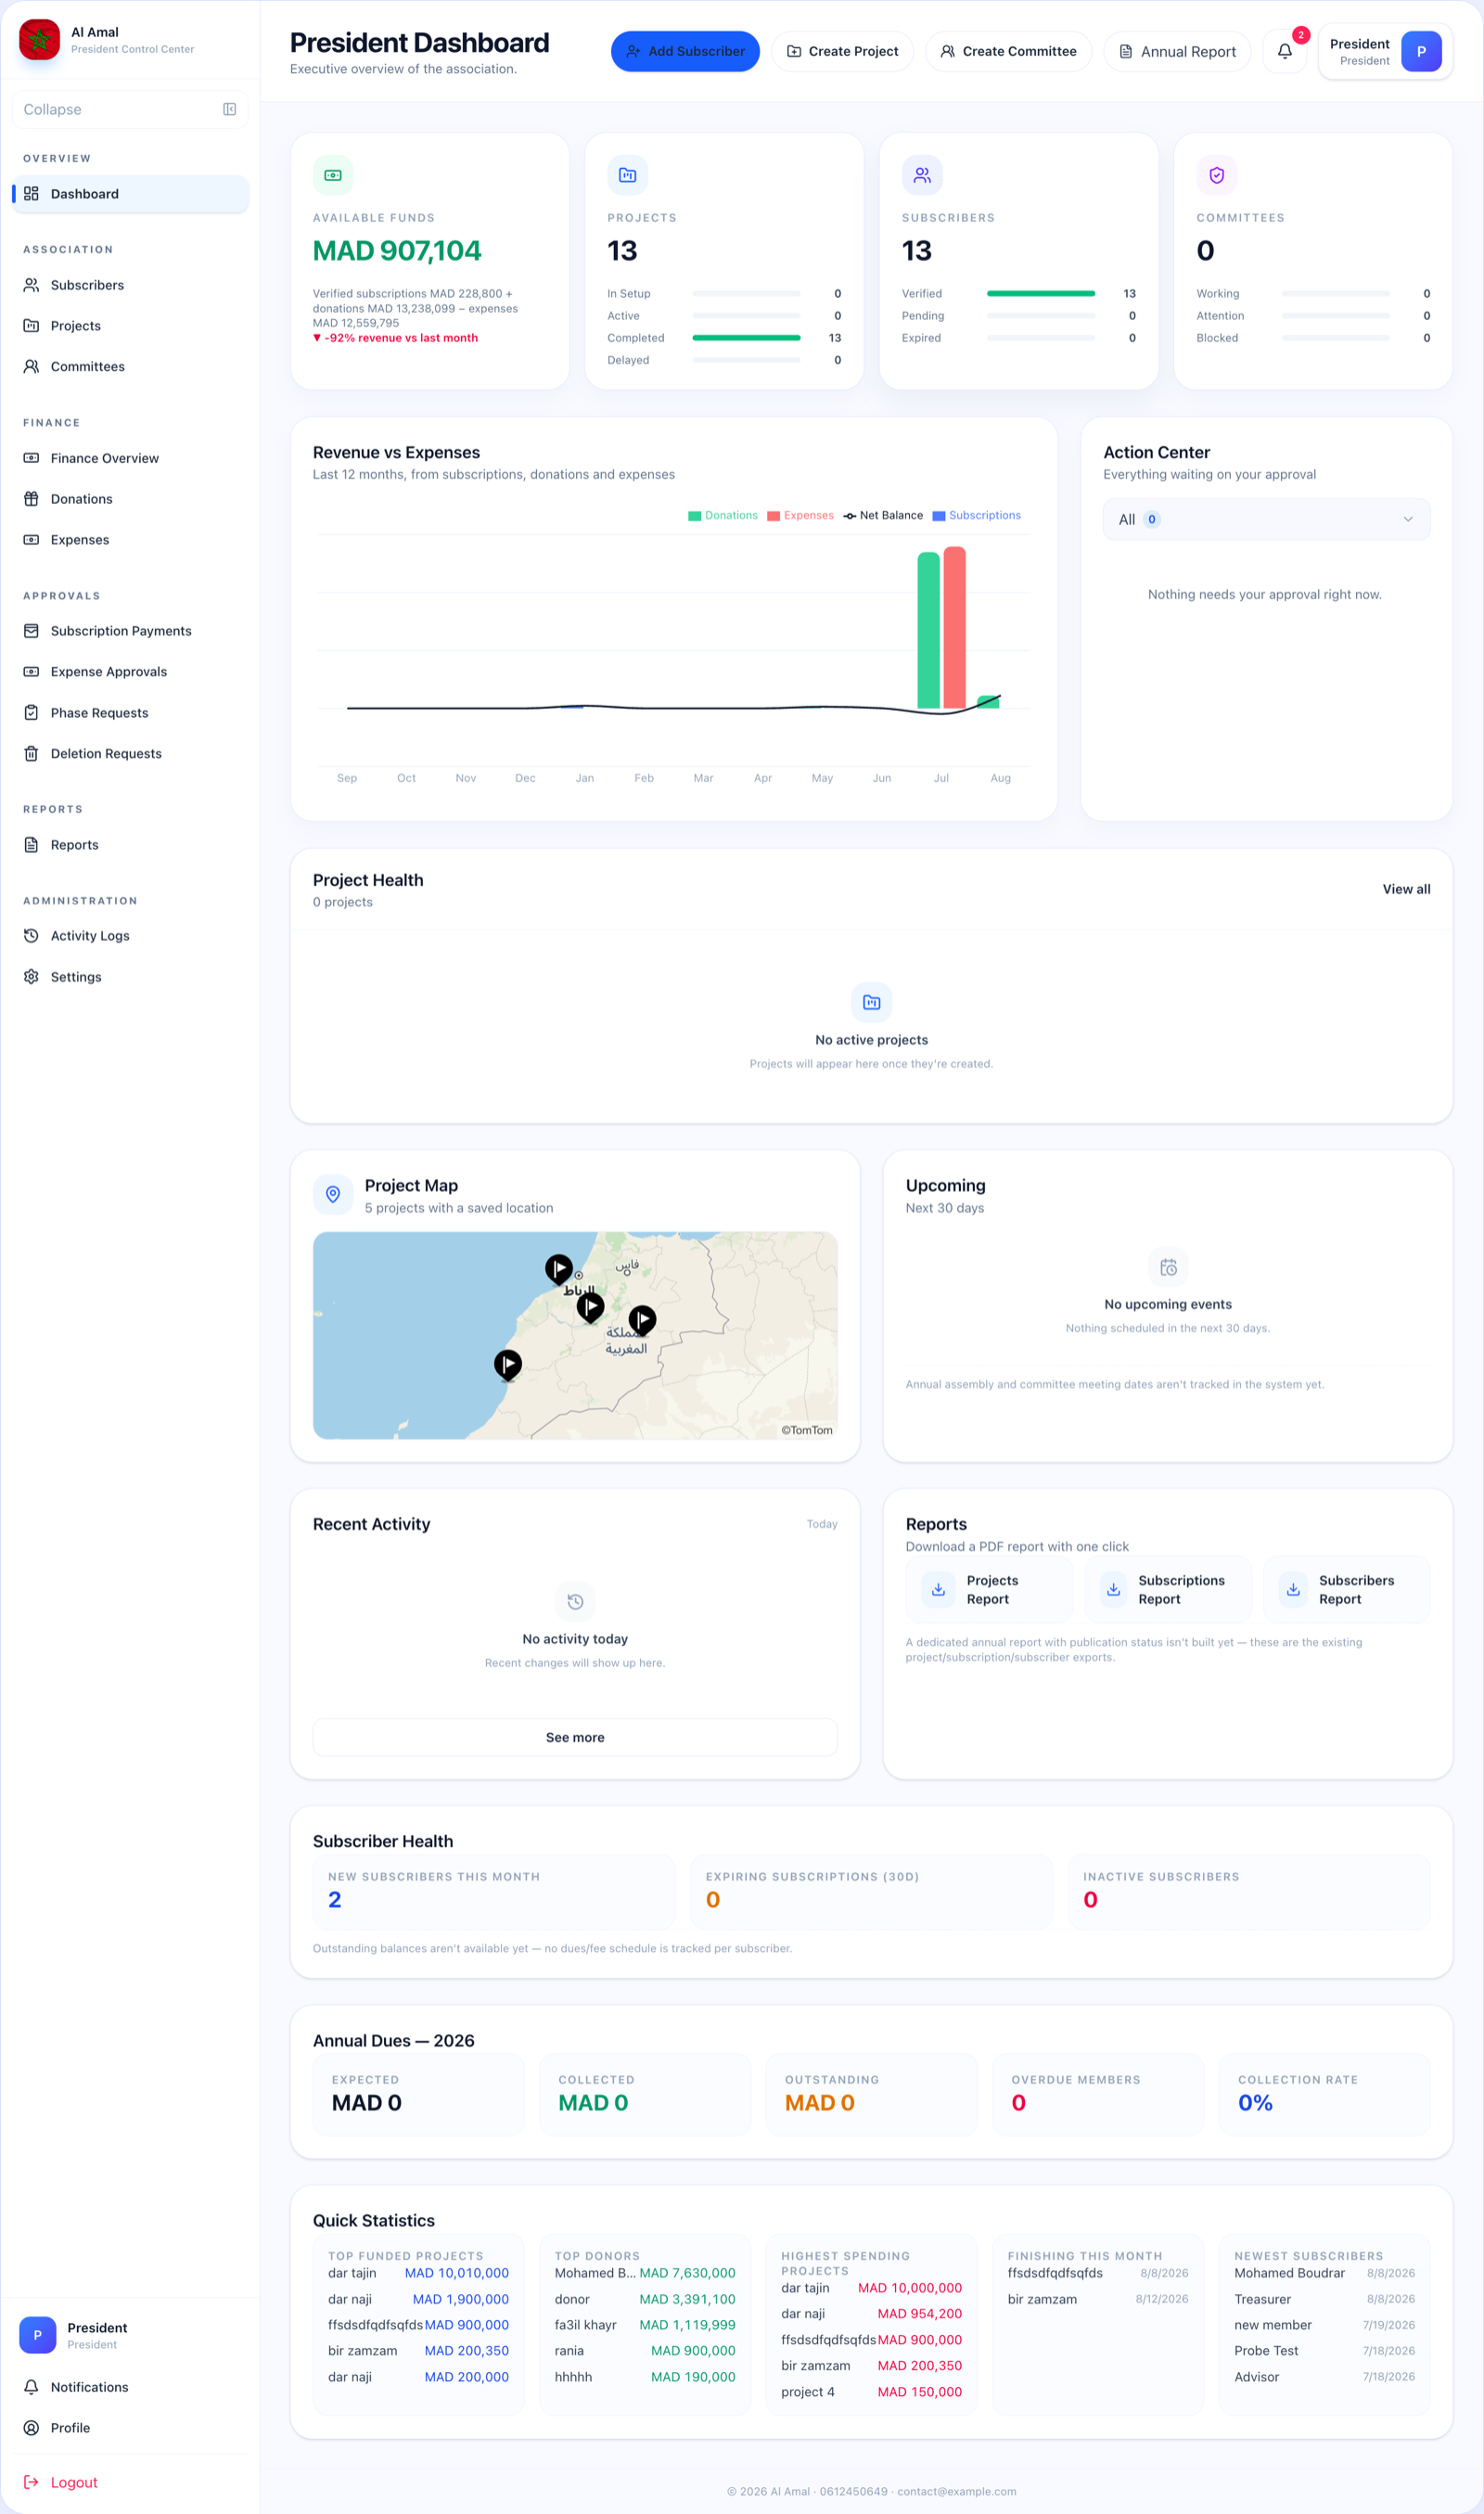
\includegraphics[width=0.92\linewidth,height=0.78\textheight,keepaspectratio]{figures/interface-dashboard.png}
  \caption{Tableau de bord du président : vue d'ensemble de l'association.}
  \label{fig:if-dashboard}
\end{figure}

\subsection{Gestion des adhérents}

Cette interface permet de créer un adhérent, de consulter et de mettre à
jour ses coordonnées, et de le supprimer.

\begin{figure}[htbp]
  \centering
  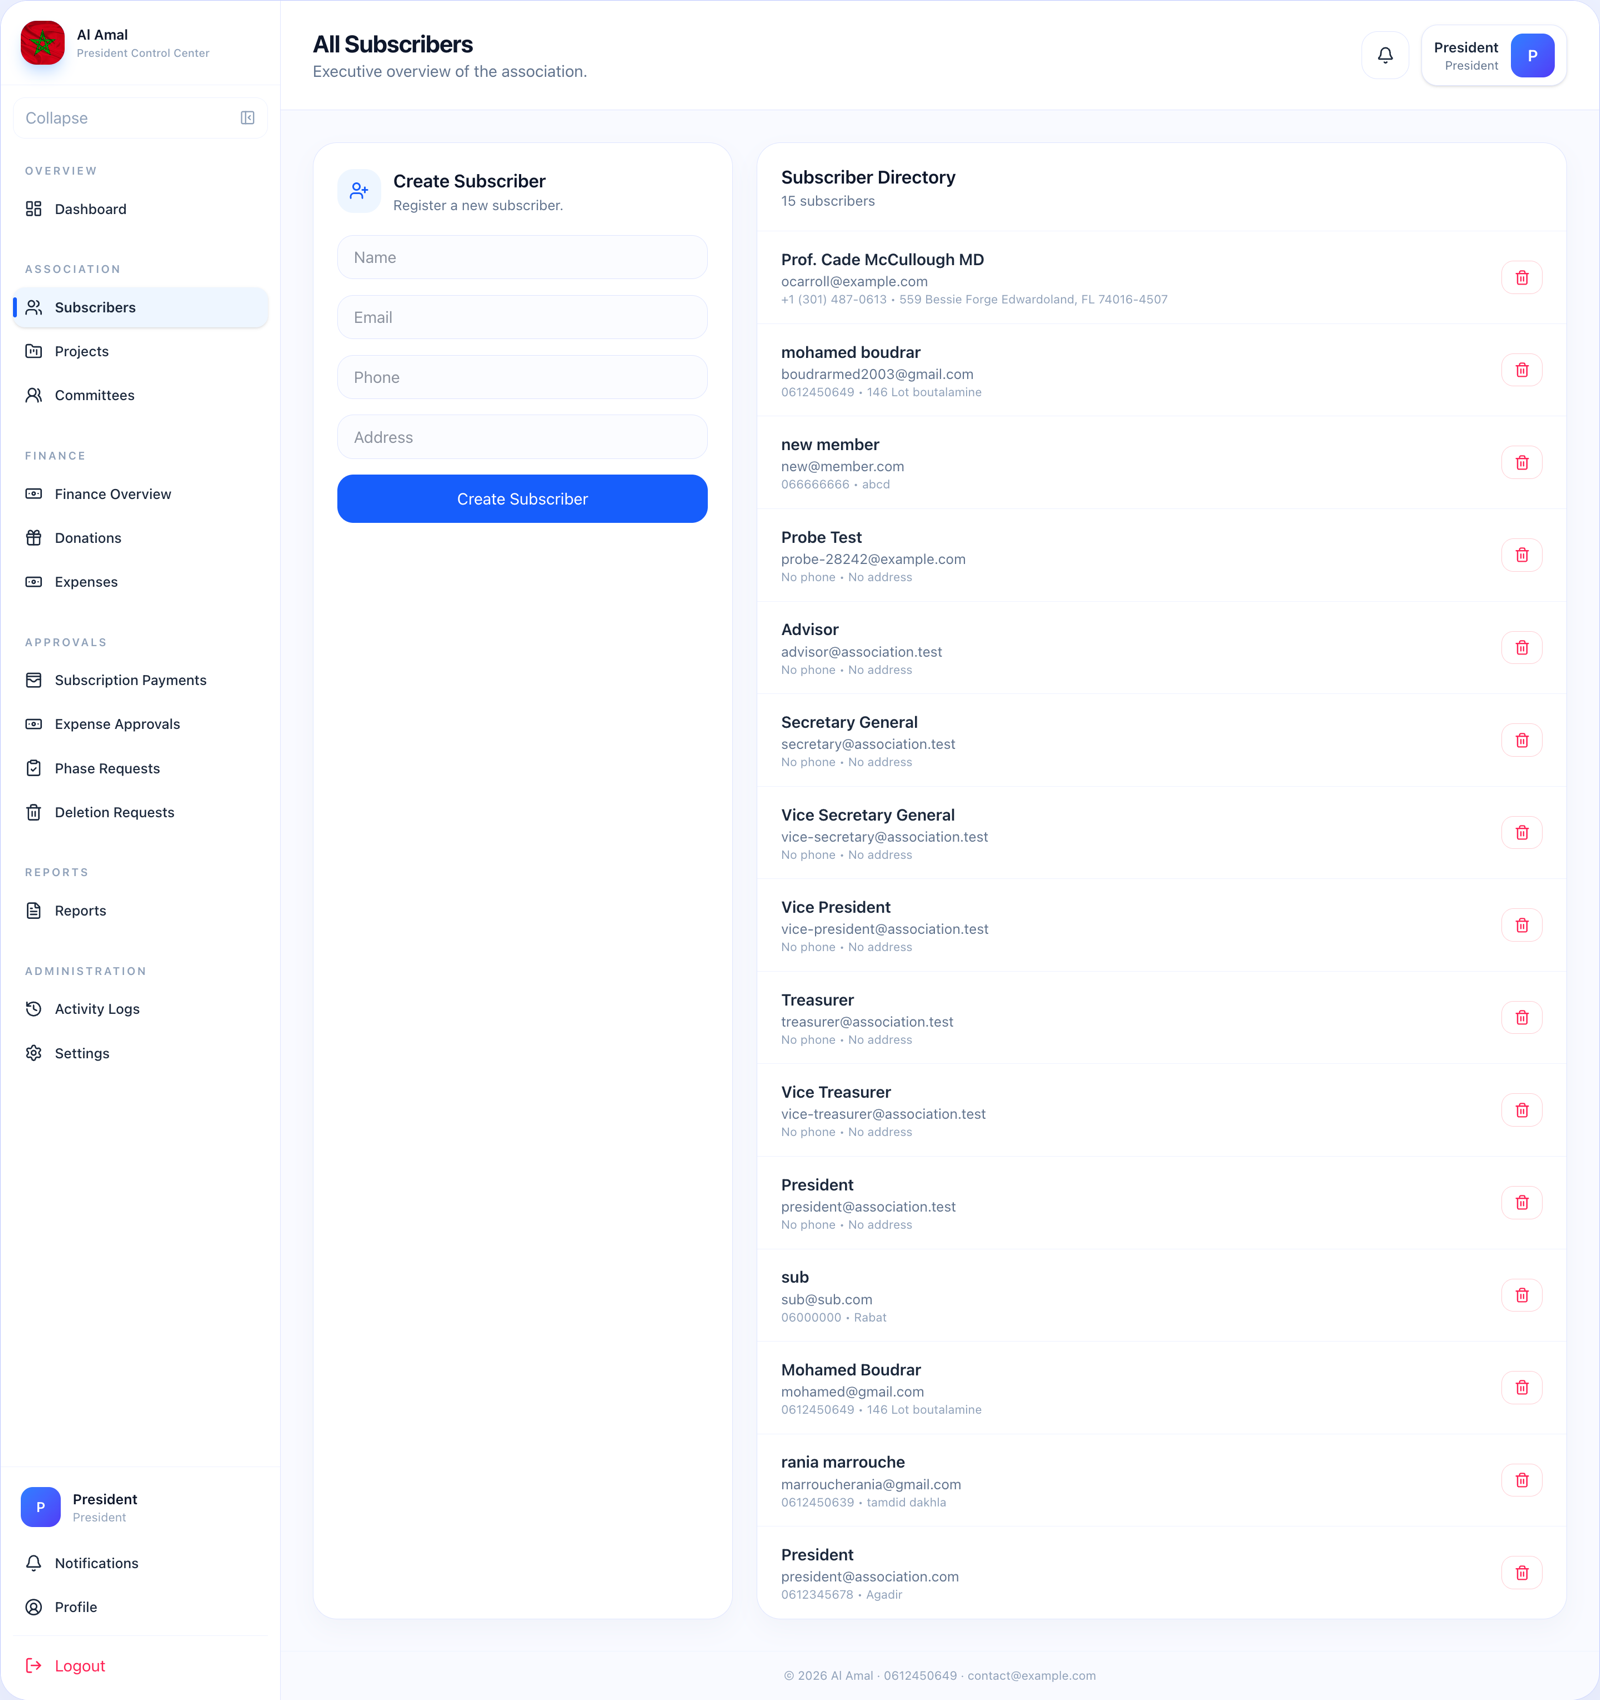
\includegraphics[width=0.92\linewidth,height=0.78\textheight,keepaspectratio]{figures/interface-membres.png}
  \caption{Gestion des adhérents.}
  \label{fig:if-membres}
\end{figure}

\subsection{Projets et comités}

La liste des projets présente leur état d'avancement ; chaque projet dispose
d'un espace de travail dédié pour son comité (figure~\ref{fig:if-projets}),
et un écran séparé permet de gérer les membres d'un comité et de consulter
son historique (figure~\ref{fig:if-comites}).

\begin{figure}[htbp]
  \centering
  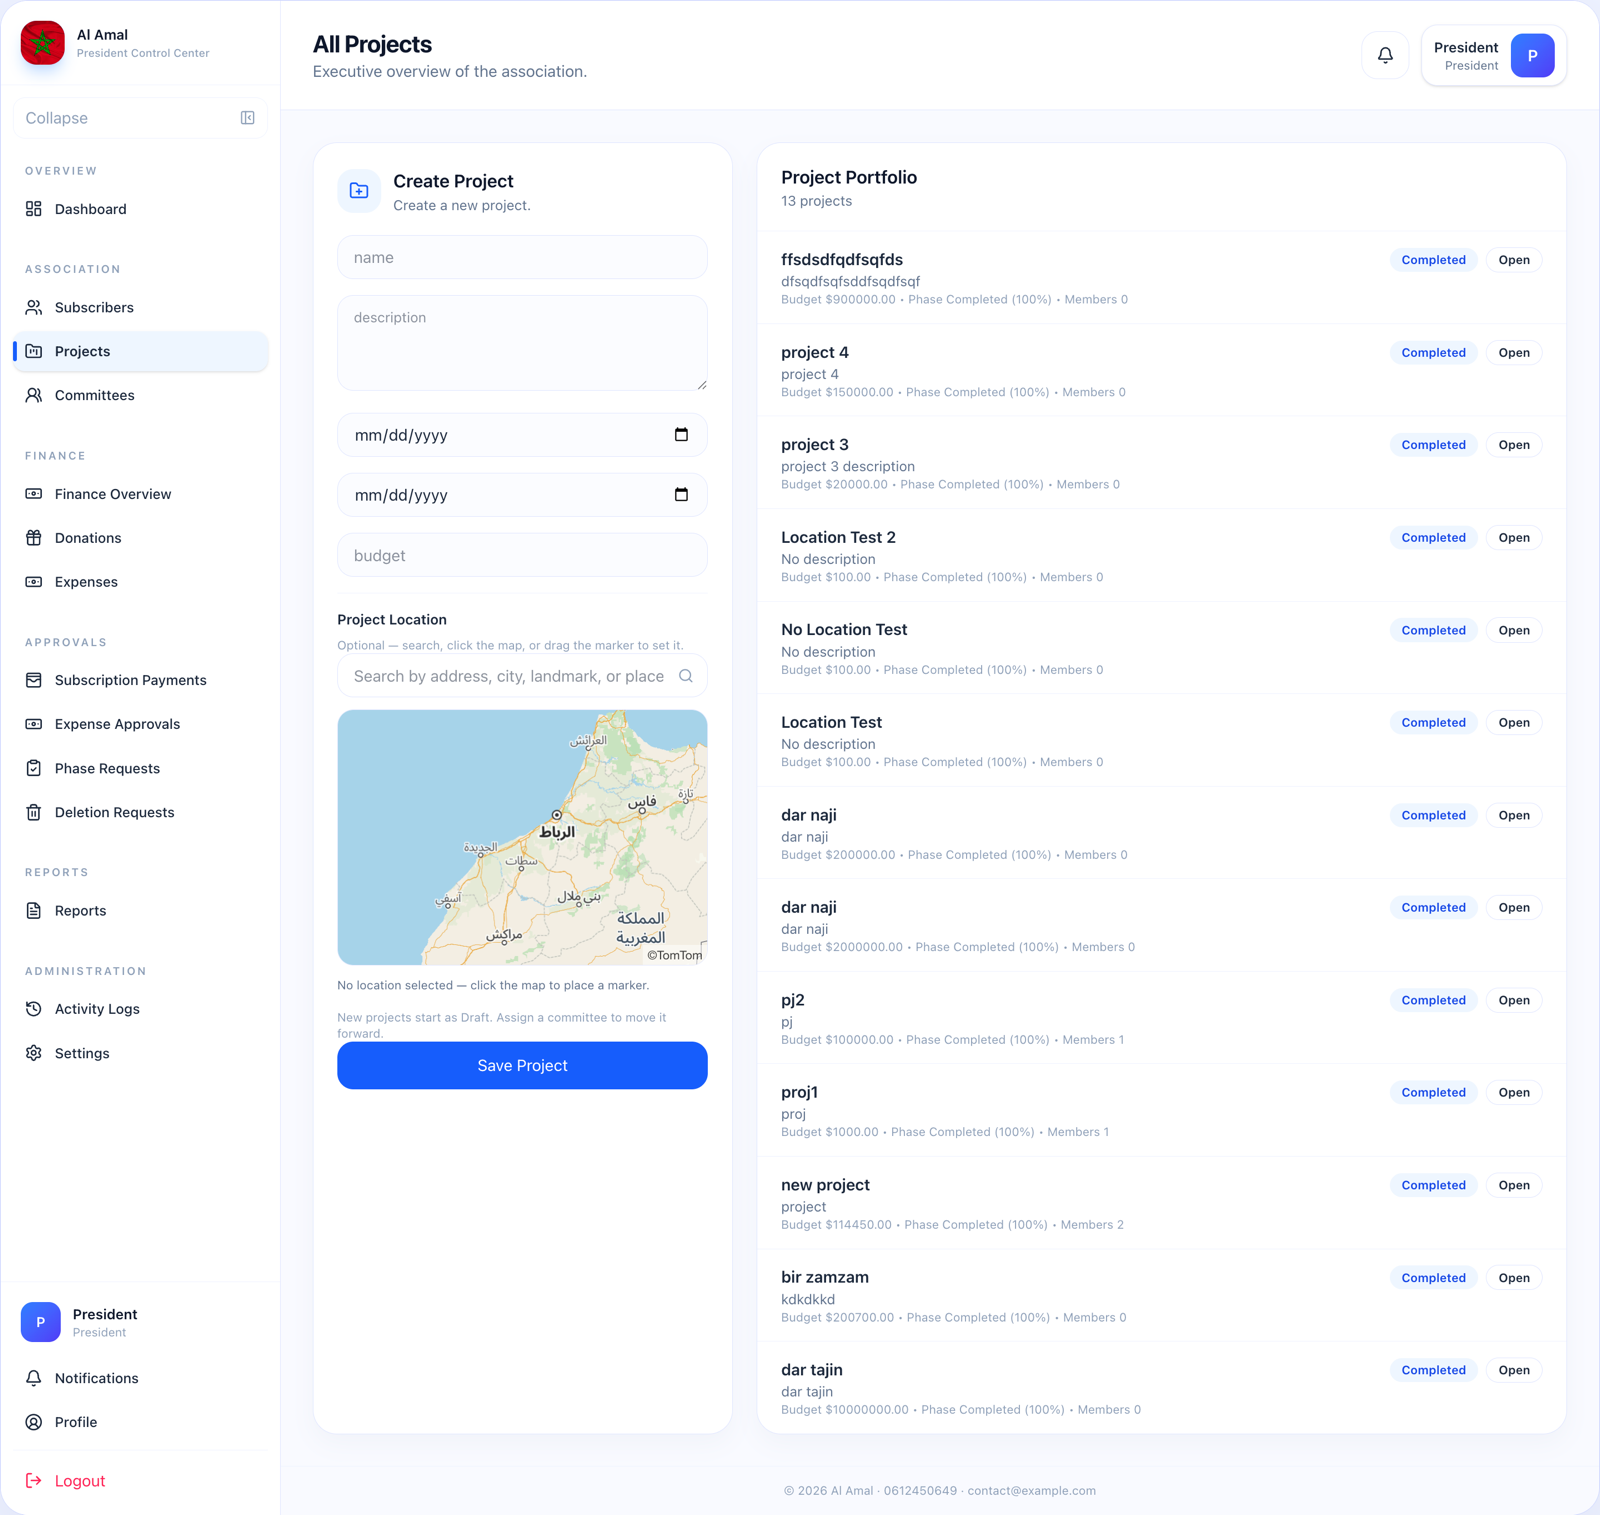
\includegraphics[width=0.92\linewidth,height=0.78\textheight,keepaspectratio]{figures/interface-projets.png}
  \caption{Liste des projets de l'association.}
  \label{fig:if-projets}
\end{figure}

\begin{figure}[htbp]
  \centering
  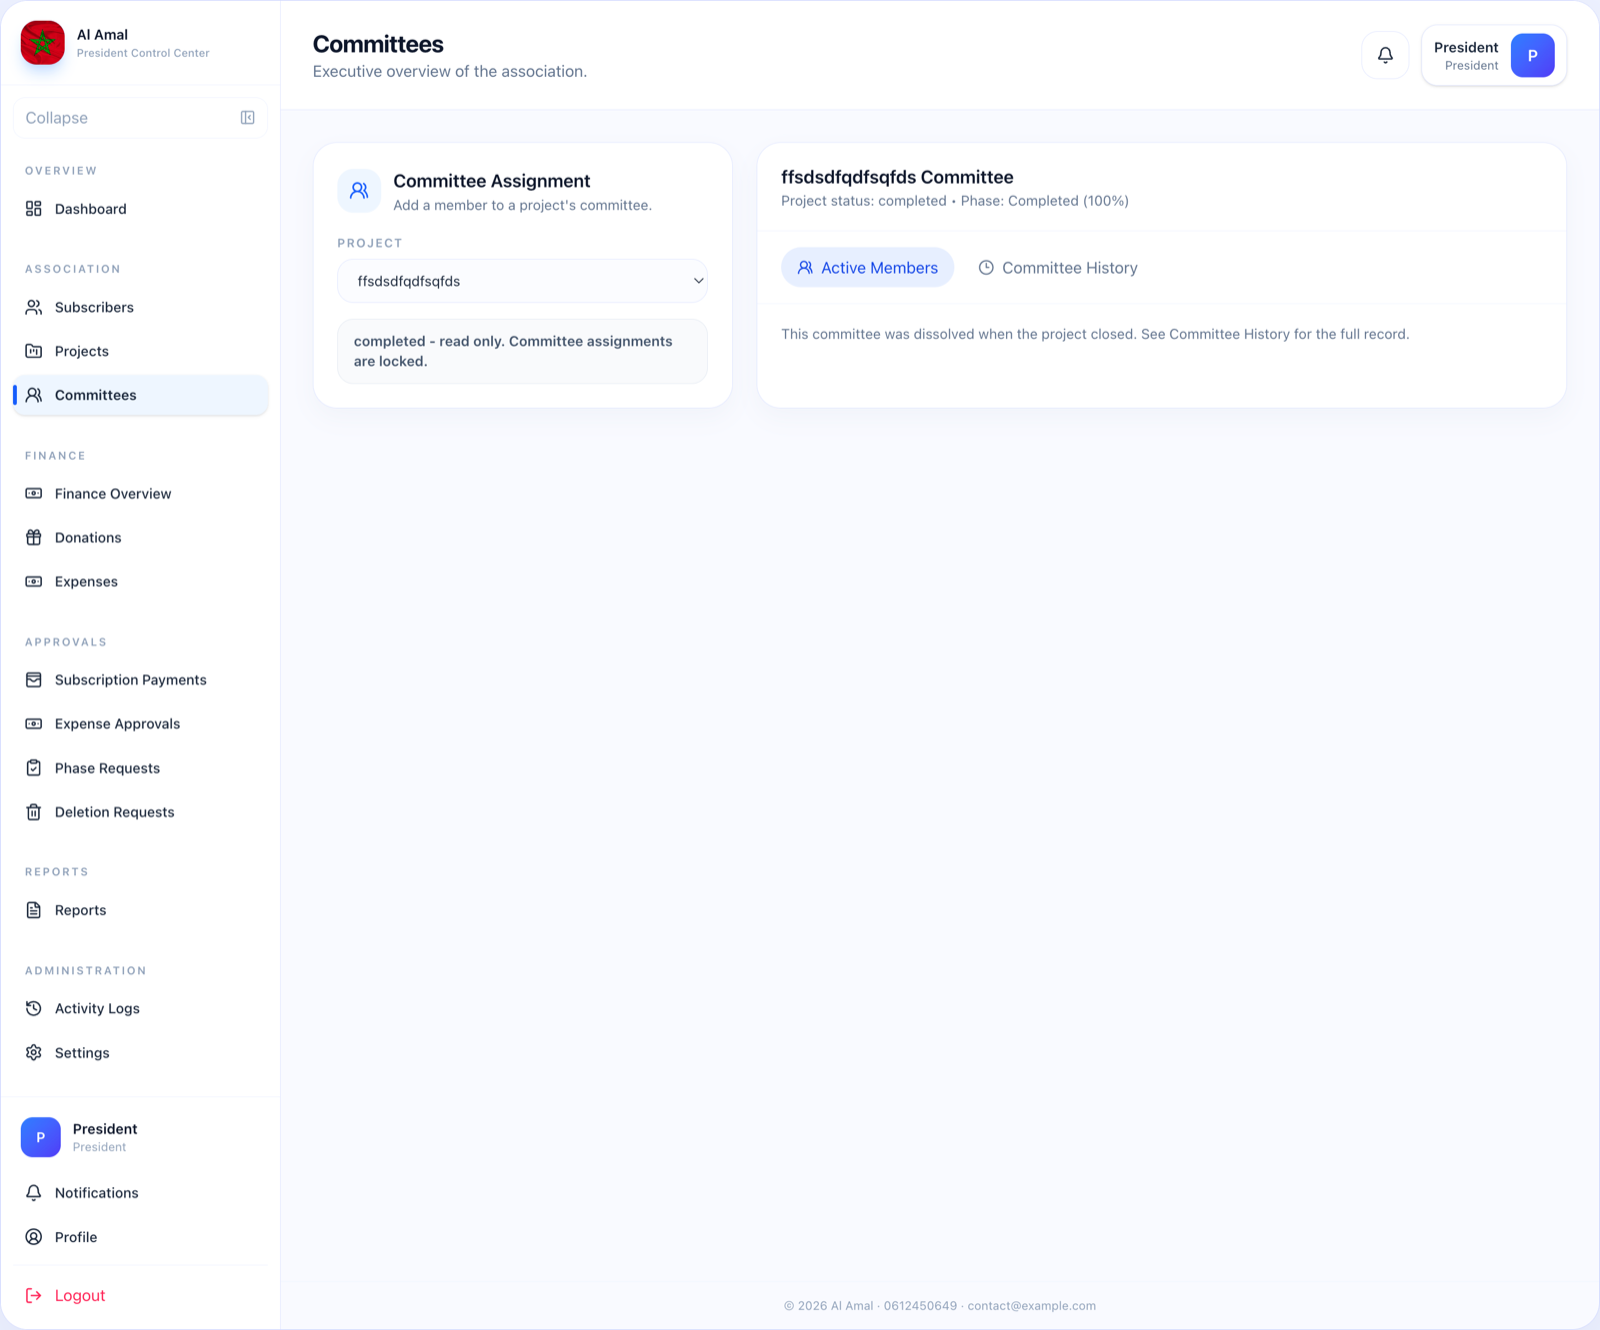
\includegraphics[width=0.92\linewidth,height=0.78\textheight,keepaspectratio]{figures/interface-comites.png}
  \caption{Gestion d'un comité de projet.}
  \label{fig:if-comites}
\end{figure}

\subsection{Finances}

L'écran des finances présente les fonds disponibles, les dons regroupés par
projet, et le financement de chaque projet (budget, dons, alloué, dépenses,
solde restant).

\begin{figure}[htbp]
  \centering
  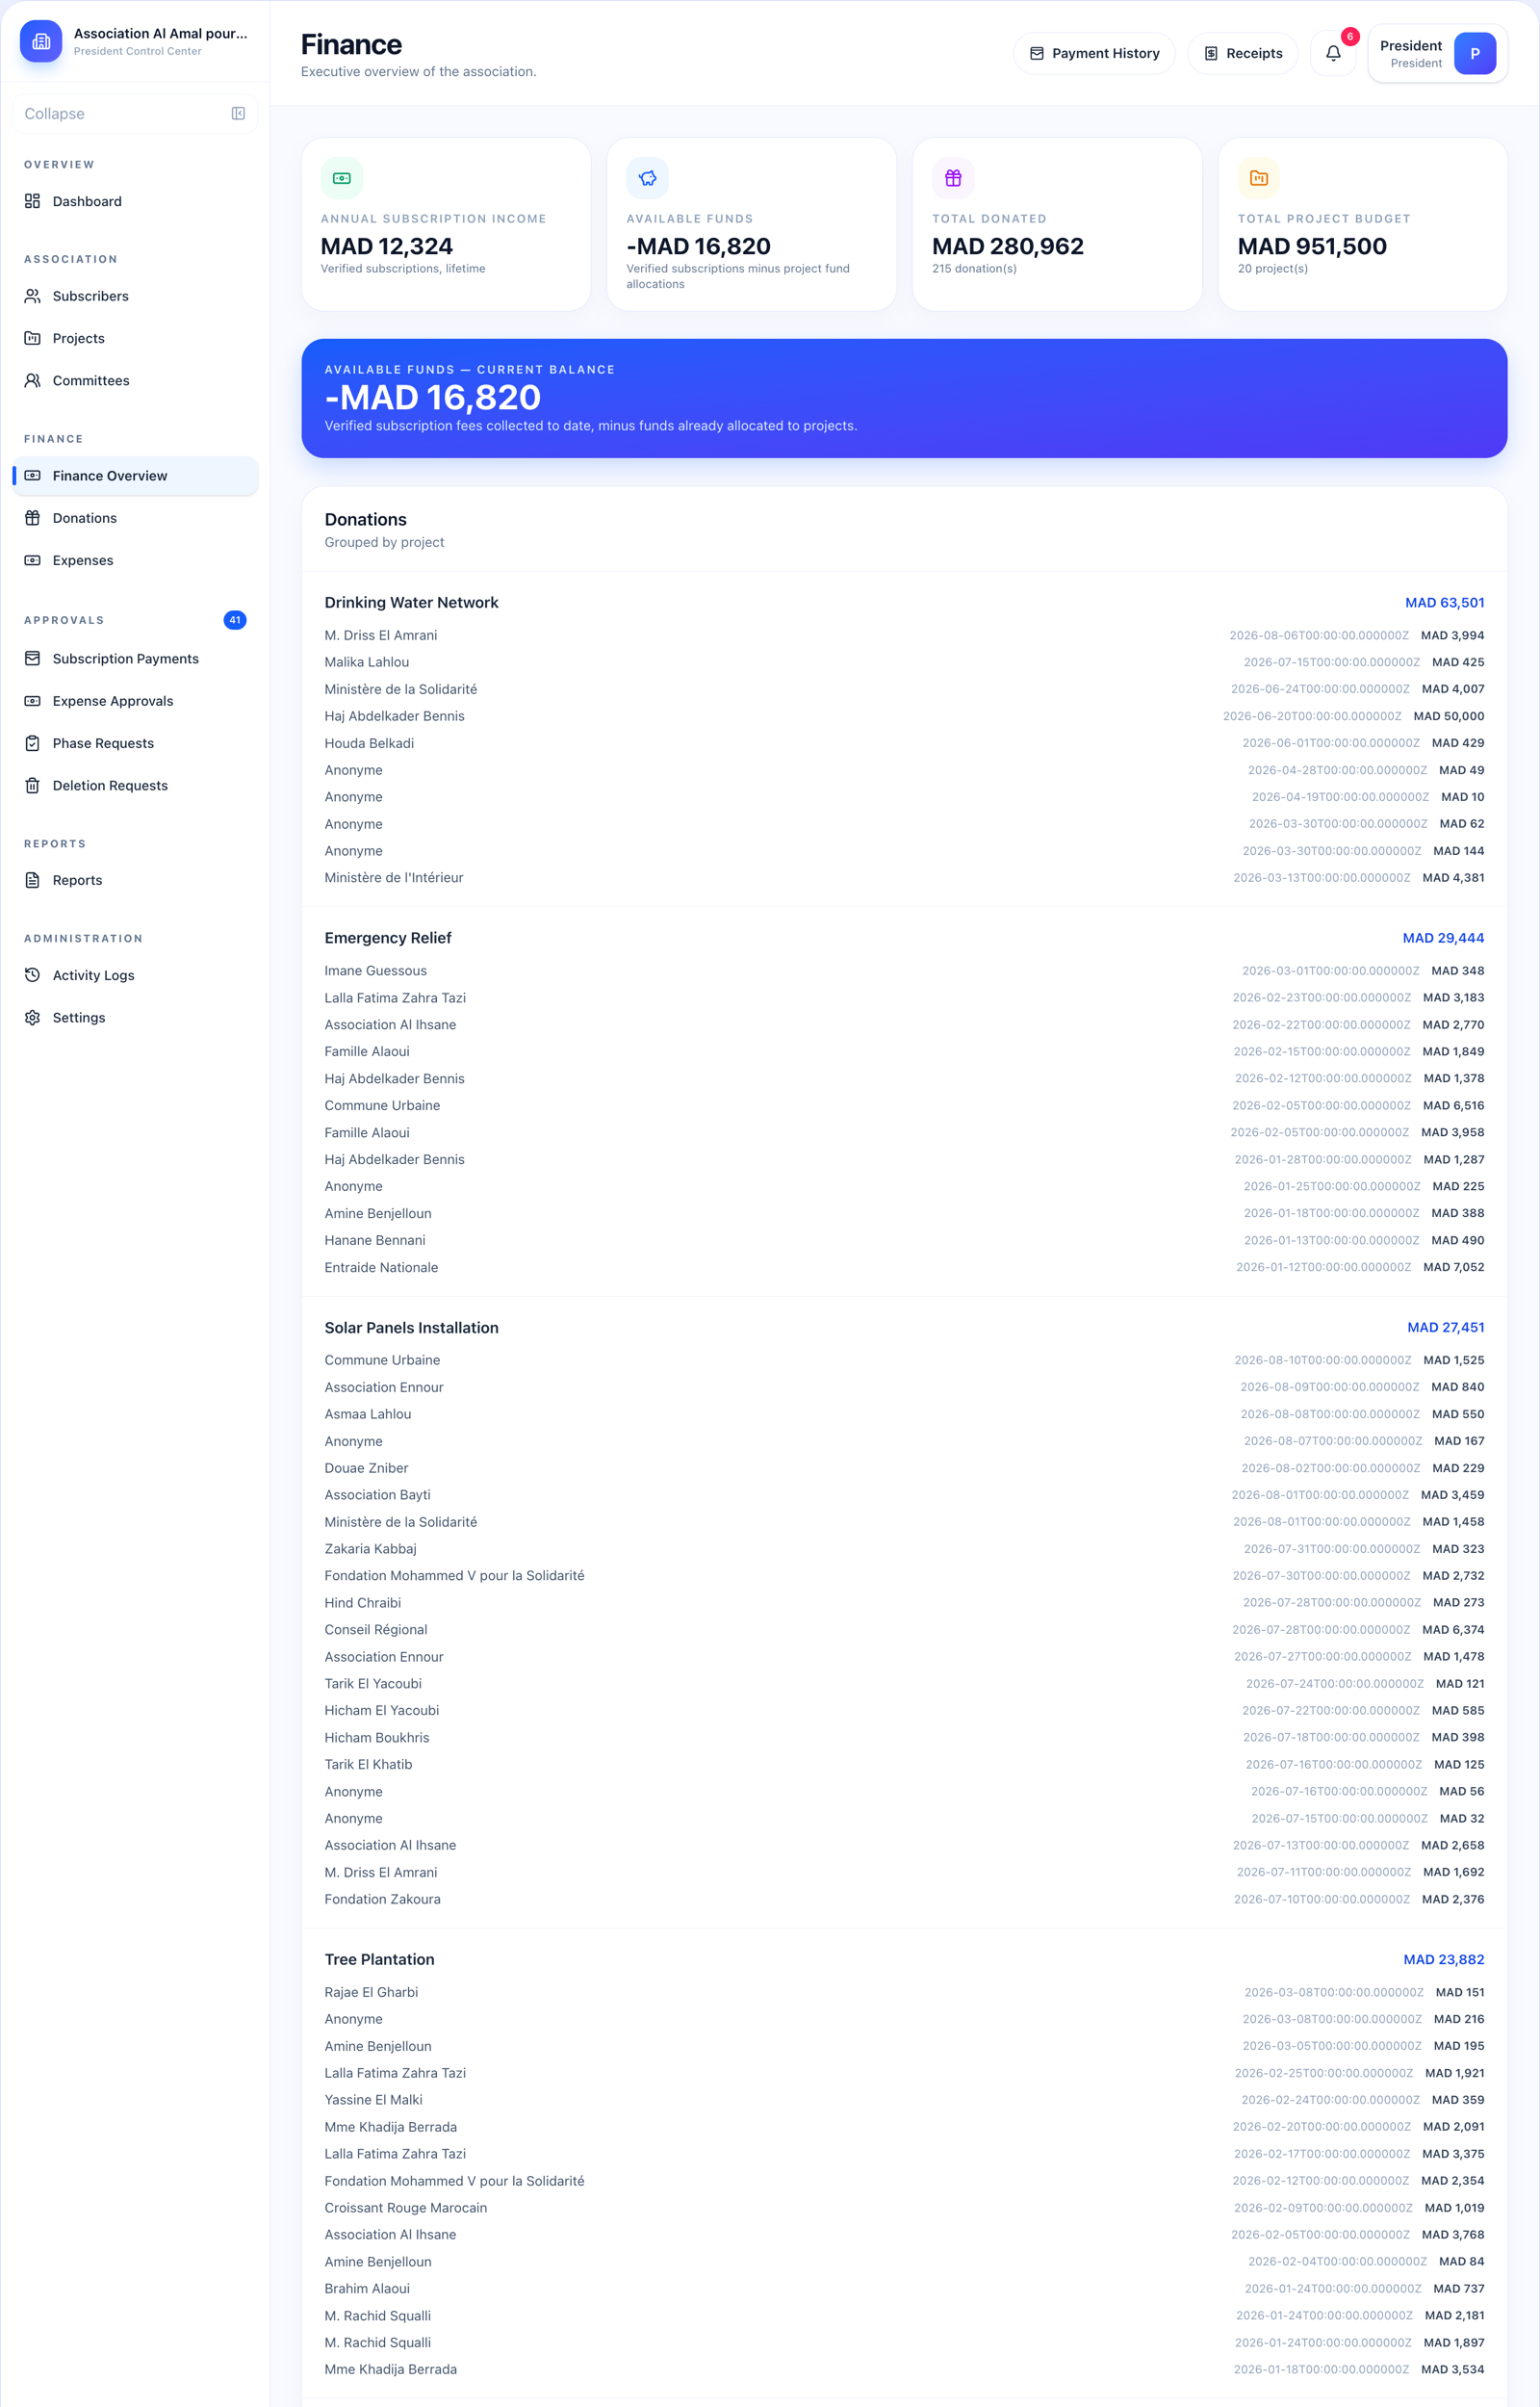
\includegraphics[width=0.92\linewidth,height=0.78\textheight,keepaspectratio]{figures/interface-finances.png}
  \caption{Vue d'ensemble des finances de l'association.}
  \label{fig:if-finances}
\end{figure}

\subsection{Approbations}

Les files d'approbation (cotisations, dons, dépenses, demandes de passage de
phase, demandes de suppression de projet) regroupent tout ce qui attend une
décision d'un rôle habilité.

\begin{figure}[htbp]
  \centering
  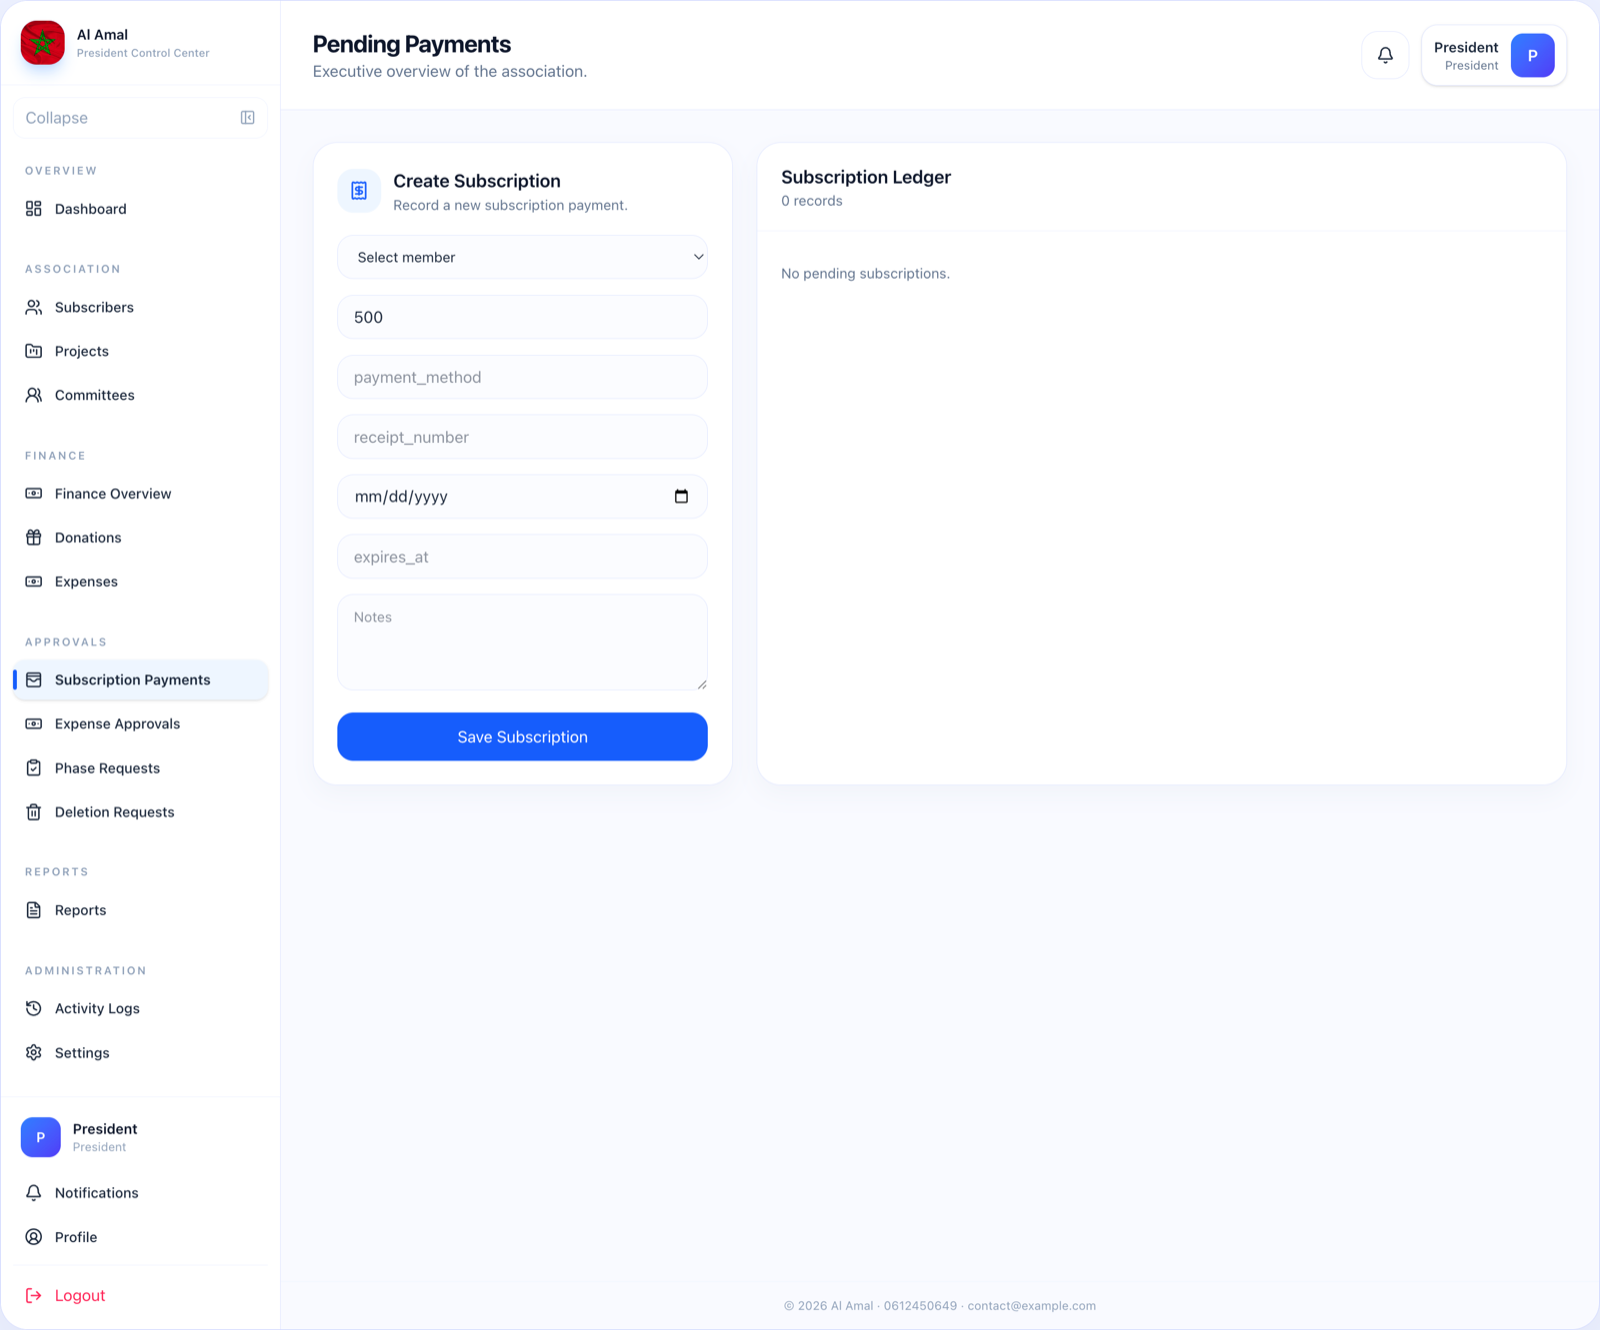
\includegraphics[width=0.92\linewidth,height=0.78\textheight,keepaspectratio]{figures/interface-approbations.png}
  \caption{File d'attente des cotisations à vérifier.}
  \label{fig:if-approbations}
\end{figure}

\subsection{Rapports}

Cet écran centralise le téléchargement des rapports association (adhérents,
cotisations, projets, cotisations dues) en PDF ou en Excel.

\begin{figure}[htbp]
  \centering
  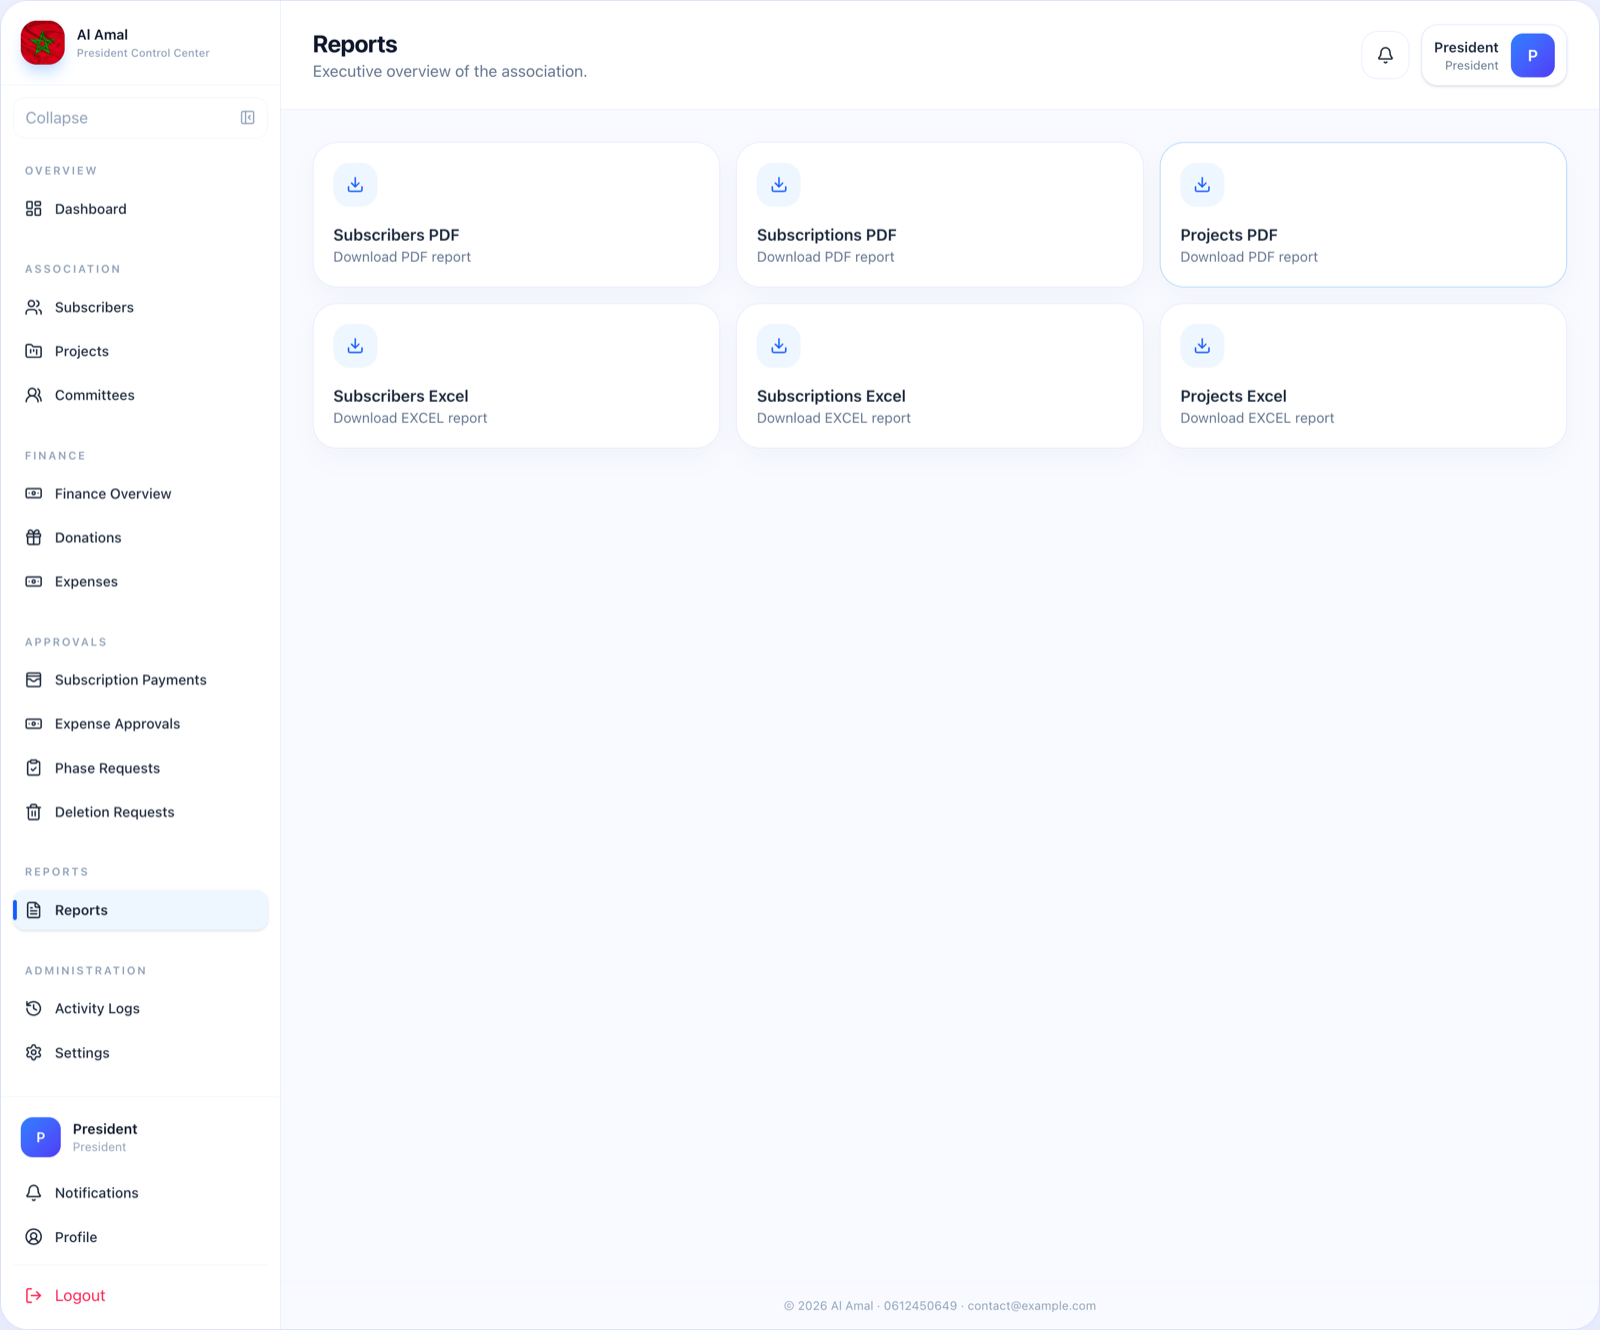
\includegraphics[width=0.92\linewidth,height=0.78\textheight,keepaspectratio]{figures/interface-rapports.png}
  \caption{Écran des rapports association.}
  \label{fig:if-rapports}
\end{figure}

\subsection{Paramètres}

Réservé au président, cet écran configure l'identité de l'association (nom,
logo, coordonnées) et le montant de la cotisation annuelle par défaut.

\begin{figure}[htbp]
  \centering
  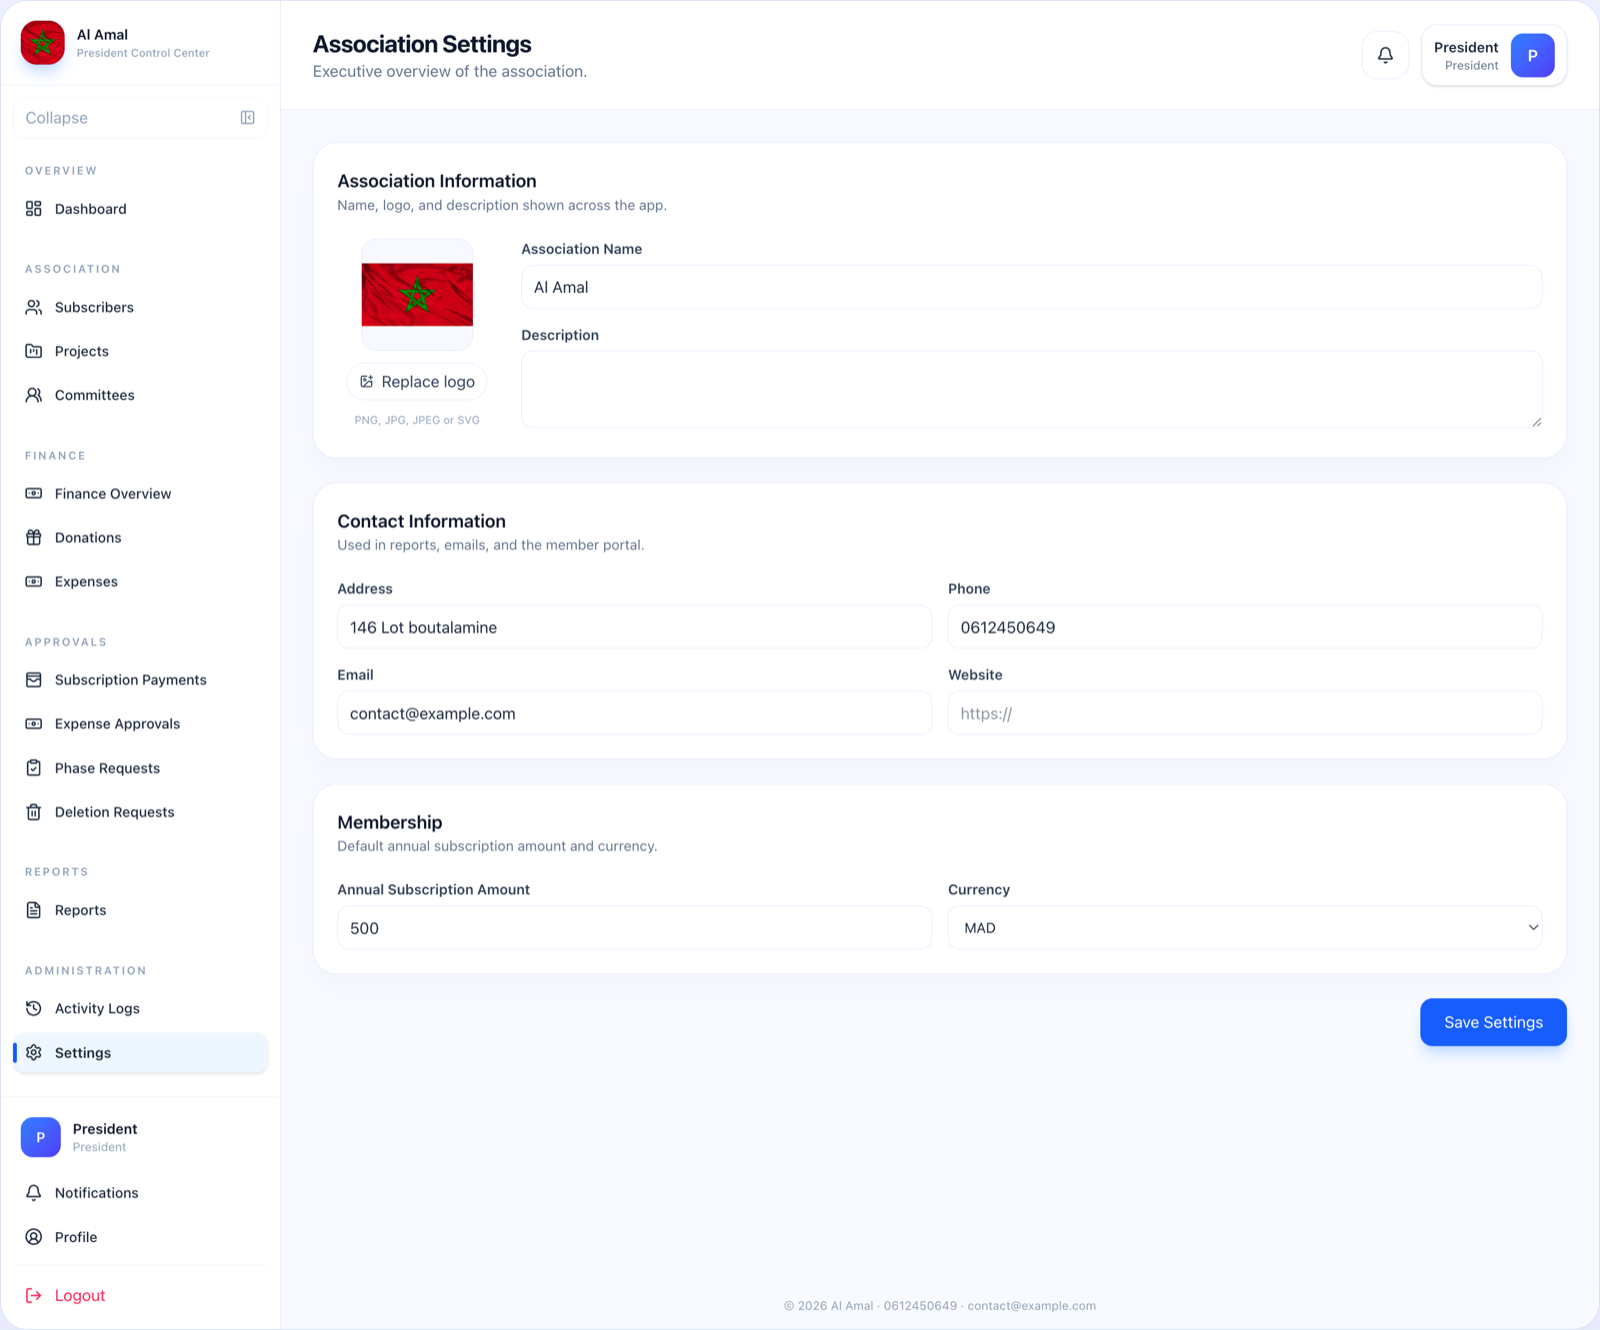
\includegraphics[width=0.92\linewidth,height=0.78\textheight,keepaspectratio]{figures/interface-parametres.png}
  \caption{Paramètres de l'association.}
  \label{fig:if-parametres}
\end{figure}

\section{Conclusion}

Ce chapitre a présenté la spécification fonctionnelle, les acteurs du système
et la structure conceptuelle des données, ainsi que l'architecture technique
retenue, l'environnement de développement, les fonctionnalités implémentées
et les interfaces développées pour chaque profil d'utilisateur.


\frontsection{Conclusion Générale}

Ce stage a permis de concevoir et de développer une plateforme web complète
de gestion associative, couvrant l'ensemble des besoins exprimés dans le
cahier des charges : gestion des adhérents et de leurs cotisations annuelles,
suivi d'un solde dû par adhérent et par année, gestion des projets
associatifs à travers un cycle de vie complet (de la création à la clôture
ou à l'annulation), constitution de comités dédiés avec des droits de saisie
propres à chaque rôle, workflow d'approbation des dons et des dépenses avec
justificatifs, génération automatique des rapports de clôture de projet et
des rapports association, journal d'activité et centre de notifications, et
consultation en libre-service par chaque adhérent de son propre historique.

Le système repose sur une architecture web en trois niveaux (interface React,
API REST Laravel, base de données MySQL), avec une autorisation à deux axes
— rôle global dans l'association et rôle au sein d'un comité de projet — qui
reflète fidèlement la manière dont une association de ce type fonctionne
réellement : un même adhérent peut être simple cotisant sur l'ensemble de
l'association et trésorier d'un comité sur un projet particulier. Cette
séparation, au cœur du cahier des charges, structure l'ensemble du modèle de
données et du système de permissions présentés au chapitre~3.

Ce projet a permis de consolider des compétences techniques en conception
d'API REST sécurisées, en modélisation de workflows métier (cycles de vie,
approbations à plusieurs états) et en développement d'interfaces web
réactives, ainsi que des compétences plus larges : traduire un besoin
métier exprimé en langage naturel en un modèle de données et un système de
permissions cohérents, et itérer sur ce modèle à mesure que des cas
particuliers apparaissent.

Plusieurs pistes d'évolution restent ouvertes pour la suite du projet :
une application mobile pour les adhérents, afin de faciliter la consultation
de leur historique et le paiement de leur cotisation ; des notifications par
SMS pour les adhérents ne disposant pas d'un smartphone ou d'un accès
régulier à internet, en complément des notifications actuelles ; et un
support multi-association, pour permettre à la même plateforme de servir
plusieurs associations indépendantes plutôt qu'une seule instance dédiée.

\frontsection{Bibliographie}

\begin{enumerate}[leftmargin=1.6cm, label={[\arabic*]}]

\item Laravel. \textit{Laravel 13.x Documentation}. \url{https://laravel.com/docs}

\item Laravel. \textit{Laravel Sanctum --- API Authentication}. \url{https://laravel.com/docs/sanctum}

\item Spatie. \textit{laravel-permission --- Associate Users with Permissions and Roles}. \url{https://spatie.be/docs/laravel-permission}

\item Spatie. \textit{laravel-activitylog --- A Very Simple Activity Logger}. \url{https://spatie.be/docs/laravel-activitylog}

\item Meta Platforms, Inc. \textit{React Documentation}. \url{https://react.dev}

\item Tailwind Labs. \textit{Tailwind CSS Documentation}. \url{https://tailwindcss.com/docs}

\item barryvdh. \textit{laravel-dompdf --- A DOMPDF Wrapper for Laravel}. \url{https://github.com/barryvdh/laravel-dompdf}

\item Maatwebsite. \textit{Laravel Excel Documentation}. \url{https://docs.laravel-excel.com}

\item Object Management Group. (2017). \textit{Unified Modeling Language (UML) Specification, Version 2.5.1}. \url{https://www.omg.org/spec/UML/2.5.1/}

\item Zietlow, J., Hankin, J. A., \& Seidner, A. (2007). \textit{Financial Management for Nonprofit Organizations: Policies and Practices}. John Wiley \& Sons.

\end{enumerate}

\frontsection{Annexes}

Cette section regroupe des documents complémentaires au rapport, trop
volumineux ou trop techniques pour figurer dans le corps du texte.

\subsection*{Annexe A : Extrait du contrat d'API --- Cotisations dues}
\addcontentsline{toc}{section}{Annexe A : Extrait du contrat d'API}

L'extrait suivant illustre la réponse de l'API pour la consultation des
cotisations dues d'un adhérent (\texttt{GET /api/dues}), et le corps de
requête pour l'exonération d'une cotisation
(\texttt{POST /api/dues/\{id\}/waive}).

\begin{lstlisting}[language=json, caption={Réponse de GET /api/dues (extrait)}, label={lst:dues-api}]
{
  "data": [
    {
      "id": 128,
      "member": { "id": 42, "name": "Adherent Test" },
      "year": 2026,
      "amount_due": 200.00,
      "amount_paid": 120.00,
      "balance": 80.00,
      "status": "partial",
      "due_date": "2026-12-31",
      "paid_at": null,
      "waived_reason": null,
      "created_at": "2026-01-01T00:30:00.000000Z"
    }
  ]
}
\end{lstlisting}

\begin{lstlisting}[language=json, caption={Corps de requête de POST /api/dues/\{id\}/waive}, label={lst:dues-waive}]
{
  "reason": "Difficulte financiere temporaire, dispense accordee par le bureau."
}
\end{lstlisting}

\subsection*{Annexe B : Matrice des rôles et des permissions}
\addcontentsline{toc}{section}{Annexe B : Matrice des rôles et des permissions}

Le tableau~\ref{tab:permissions} reproduit la matrice complète des droits
accordés à chacun des huit rôles globaux, telle qu'implémentée dans le
système de permissions (Spatie Permission). \emph{view}/\emph{create}/
\emph{update}/\emph{delete}/\emph{verify} correspondent aux opérations
autorisées sur chaque type de ressource.

\begin{center}
\begin{longtable}{@{}p{2.6cm}p{2.1cm}p{2.9cm}p{1.2cm}p{2.1cm}p{2.4cm}p{2.4cm}@{}}
\toprule
\textbf{Rôle} & \textbf{Adhérents} & \textbf{Cotisations} & \textbf{Dues} & \textbf{Projets} & \textbf{Dons} & \textbf{Dépenses} \\
\midrule
\endhead
Président & view/create/\allowbreak update/delete & view/create/\allowbreak update/delete/\allowbreak verify & view & view/create/\allowbreak update/delete & view/create/\allowbreak update/delete & view/create/\allowbreak update/delete \\
Vice-président & view/update & view & view & view/create/\allowbreak update & view/create/\allowbreak update & view/create/\allowbreak update \\
Trésorier & view & view/create/\allowbreak update/verify & view & view & view/create/\allowbreak update/delete & view/create/\allowbreak update/delete \\
Vice-trésorier & view & view/verify & view & view & view/create/\allowbreak update/delete & view/create/\allowbreak update/delete \\
Secrétaire général & view/create/\allowbreak update & view & view & view & view/create/\allowbreak update & view/create/\allowbreak update \\
Vice-secrétaire général & view/update & view & view & view & view/create/\allowbreak update & view/create/\allowbreak update \\
Conseiller & view & view & view & view & view/create/\allowbreak update & view/create/\allowbreak update \\
Adhérent (abonné) & vue propre uniquement & vue propre uniquement & vue propre uniquement & projets du comité uniquement & --- & --- \\
\bottomrule
\caption{Matrice des rôles et des permissions.}
\label{tab:permissions}
\end{longtable}
\end{center}

À ces permissions globales s'ajoute, indépendamment, le rôle de comité
(président de comité, trésorier, secrétaire, membre) décrit au
chapitre~3 (section~III), qui gouverne la saisie des opérations
\emph{à l'échelle d'un projet donné}, quel que soit le rôle global du
membre.

\subsection*{Annexe C : Schéma de base de données (synthèse)}
\addcontentsline{toc}{section}{Annexe C : Schéma de base de données}

Le tableau~\ref{tab:schema} résume les principales tables du schéma
relationnel et leurs colonnes clés.

\begin{center}
\begin{longtable}{@{}p{3.3cm}p{10.8cm}@{}}
\toprule
\textbf{Table} & \textbf{Colonnes clés} \\
\midrule
\endhead
\texttt{users} & name, email, password, passkey\_hash \\
\texttt{members} & user\_id, phone, address \\
\texttt{subscriptions} & member\_id, due\_id, amount, payment\_method, receipt\_number, payment\_date, expires\_at, status, verified\_by, verified\_at \\
\texttt{dues} & member\_id, year, amount\_due, amount\_paid, balance, status, due\_date, paid\_at, waived\_reason (unique sur member\_id + year) \\
\texttt{projects} & name, description, start\_date, end\_date, budget, status, phase, latitude, longitude, manager\_id \\
\texttt{member\_project} & member\_id, project\_id, committee\_role, responsibility, assigned\_by, assigned\_at \\
\texttt{committee\_assignments} & project\_id, member\_id, committee\_role, assigned\_by/at, removed\_by/at, reason, action \\
\texttt{donations} & member\_id, project\_id, donor\_name, amount, payment\_method, receipt\_number, donation\_date, status, approved\_by/at, rejected\_by/at, rejection\_reason, rejection\_type \\
\texttt{expenses} & project\_id, supplier\_name, description, amount, payment\_method, invoice\_number, expense\_date, status, approved\_by/at, rejected\_by/at, paid\_by/at \\
\texttt{project\_fund\_allocations} & project\_id, amount, allocation\_date, proof\_file, recorded\_by \\
\texttt{project\_reports} & project\_id, generated\_by, file\_path, summary (JSON) \\
\texttt{notifications} & user\_id, type, title, message, subject\_type, subject\_id, read\_at \\
\texttt{association\_settings} & association\_name, address, phone, email, annual\_subscription\_amount, currency \\
\bottomrule
\caption{Synthèse du schéma de base de données.}
\label{tab:schema}
\end{longtable}
\end{center}


\end{document}
